\documentclass[a4paper,12pt]{article}
\usepackage{natbib}
\usepackage{times}
\usepackage{amsmath}
\usepackage{amsfonts}
\usepackage{amsthm}
\usepackage{graphicx}
\usepackage{listings}
\usepackage{color}
\usepackage{nameref}
\usepackage{caption}
\usepackage{subcaption}
\usepackage{hyperref}

\usepackage[utf8]{inputenc}



\usepackage{geometry}
 \geometry{
 a4paper,
 left=30mm,
 top=25mm,
 right=15mm,
 bottom=25mm,
 }

\renewcommand{\baselinestretch}{1.5}

\bibliographystyle{apalike}






\definecolor{dkgreen}{rgb}{0,0.6,0}
\definecolor{gray}{rgb}{0.5,0.5,0.5}
\definecolor{mauve}{rgb}{0.58,0,0.82}

\lstset{ 
       language=Octave, 
       morecomment = [l][\itshape\color{blue}]{\%} 
    } 

\lstset{frame=tb,
  language=Python,
  aboveskip=3mm,
  belowskip=3mm,
  showstringspaces=false,
  columns=flexible,
  basicstyle={\small\ttfamily},
  numbers=none,
  numberstyle=\tiny\color{gray},
  keywordstyle=\color{blue},
  commentstyle=\color{dkgreen},
  stringstyle=\color{mauve},
  breaklines=true,
  breakatwhitespace=true,
  tabsize=3
}




\newtheorem{theorem}{Theorem}[section]
\theoremstyle{definition}
\newtheorem{definition}{Definition}[section]

\graphicspath{ {graphs/} }


\title{\textbf{Applications of Homogeneous Markovian Processes in Economics and Latent Parameters Estimation for Discrete State Hidden Markov Models}}
\author{\textit{Student}: Adrian Vrabie \href{adrian@vrabie.net}{adrian@vrabie.net}\\
		\textit{Academic Adviser}: Dr. habil. Dmitrii Lozovanu, University Professor \\
\href{lozovanu@math.md}{lozovanu@math.md}}
\date{\today}




\begin{document}
\maketitle
\begin{abstract}
Markovian processes are already ubiquitous in a wide range of real world applications and serendipitously provide remarkable goodness of fit despite its simplistic mathematical model.  The more general Hidden Markov Model presents difficulties when estimating its parameters therefore limiting its widespread adoption by industry and academia. This thesis addresses this issue by surveying algorithms useful for estimating matrix coefficients of HMMs. 
The first part commences with an introduction to simple Markovian processes and their applications in economics. The second part elaborates on methods and algorithms of the EM class for estimating latent state transition probabilities of Hidden Markov Models. 
Once the transition probability matrix is determined we can use the dynamic programming and combinatorial methods proposed by \cite{Lozovanu15} for determining the state-time probabilities and the matrix of limiting probabilities in solving real world questions.

Software implementations in Octave, Python and Julia are provided based on the open-source QuantEcon  and GHMM packages.

\end{abstract}
\newpage
\tableofcontents
\newpage
\listoffigures



\newpage
\setcounter{secnumdepth}{0}
\section{Acknowledgements}
\setcounter{secnumdepth}{1}
First of all I would like to express my deepest appreciation to my academic adviser Prof Dr. Habil Dmitrii Lozovanu for his invaluable advise, inspiration and lectures on Markov Chains. He convincingly conveyed a passion for research which sparked my interest in pursuing Markovian processes.

Secondly I want to render my deepest gratitude to Prof Alexandra Tkacenko for her input and for her support. If not for her lectures I would have never fully understood the beauty of optimizations in HMM for parameter estimation. 

I would also like to thank Prof Viorel Grigorcea and Prof Valeriu Gutu for administrative support. Their selfless time and care were sometimes all that kept me going.
Many thanks to Drd MD Nadeja Negari for taking care of my health and the fact that she started sharing my interest in pursuing applications of Markov chains in genetics and restlessly supported me in every endeavour.  To Mr Dorin Vremis for his inspiration in pursuing academic goals and for borrowing me a sense of humour when I lost mine. 

I am much indebted to my colleagues from work for their care and encouragement in writing my thesis: Eduard Calancea, Galina Buga and Victoria Minciuc. Sometimes they were more worried than I was about my deadlines and outcomes.

I would like to thank in advance the Examining Committee for their patience and questions and the whole faculty of Mathematics and Computer Science from the State University of Moldova. 

Many thanks to my colleagues for their input and encouragement and not least I would like to thank You, the reader, whoever you are. 
\newpage
\setcounter{secnumdepth}{0}
\section{Preface}
\setcounter{secnumdepth}{1}

The question that sparked my interest in studying Markovian processes is how to estimate the parameters of a HMM. In particular, given a set of observations, how to find the best estimates for the state transition stochastic matrix $\mathbb{A}$.

Markovian processes are ubiquitous in many real world applications, including algorithmic music composition, the Google search engine\footnote{see: \cite{langville2011google} and \cite{Stachurski2008}, }, asset pricing models, information processing, machine learning, computer malware detection \footnote{For computer viruses and malware detection using Hidden Markov Models, see \citep{lin2011hunting} } and many more.\footnote{ see speech: \href{http://www.math.harvard.edu/~kmatveev/markov.html}{http://www.math.harvard.edu/~kmatveev/markov.html}} Markov chains can be used to help model how plants grow, chemicals react, and atoms diffuse and applications are increasingly being found in such areas as engineering, computer science, economics, and education. Jeffrey Kuan at Harvard University claimed that Markov chains not only had a tremendous influence on the development of mathematics, but that Markov models might well be \textbf{ the most \textit{"real world"} useful mathematical concept after that of a derivative.}

As we will see, Markovian chains and Hidden Markov Models have a rich yet accessible mathematical texture and have become increasingly applicable in a wide range of applications. Although the assumptions underpinning Markovian processes can be perceived as unacceptably restrictive at first, Markov models tend to fit the data particularly well. To fast-forward the conclusions of this thesis, it all gets down to how well we define what \textit{a state} is. Also, there are many types of Markovian processes each with its set of particular features. In this paper we deal with only one particular class: the models that exhibit time invariant probability distributions within a state.\footnote{Analogous to difference equations, we are not interested in the systems dependent on time $t$ as this will exponentially complicate our estimation technique.} These models allow the use of the theoretical results from studies focused on the convergence properties of stationary  distribution as time $t \mapsto \infty$. This is of use in Economics because it opens avenues not only to reinterpret economic growth in the settings of a stochastic matrix but allows to efficiently compute expected long-term economic growth rates.  

The extension of Markovian chains to HMMs allows modelling even a wider scope of applications, suitable not only to describing the behaviour of the economy at a macroeconomic level but also for monetary policy advise. This can resolve the Morgenstern's critique. \footnote{In his book, On the Accuracy of Economic Observations (1950), Morgenstern expressed his concerns in the way the data is used from the national income accounts to reach conclusions about the state of the economy and about appropriate policies. Note for Mathematicians: Morgenstern was a friend of John von Neumann.} Also, as one of the leading graduate Economics textbook puts it "Understanding the causes of aggregate fluctuations is the central goal of macroeconomics"\cite{Romer06}. Moreover, \cite{Romer06}[Ch4, pp.174] notes "A first important fact about fluctuations is that they do not exhibit any simple regular or cyclical pattern." Markov Chains substantially improve the prediction of the macroeconomic aggregates when compared to time series techniques, such as ARIMA models. Moreover, as shown by \cite{Tauchen86} we can pretty accurately approximate an ARMA process with a Markov Chain given enough states.


A broadly applicable algorithm for computing maximum likelihood estimates from incomplete data is the EM algorithm, see {Dempster77}. The work of \cite{Dempster77} was based on the Ph.D. thesis of \cite{sundberg1972maximum} which provided a very detailed treatment of the EM method for exponential functions. 
 The first to describe this EM algorithm in the paradigm of a mathematical maximization technique for probabilistic functions in Markov chains was \cite{baum1970maximization}\footnote{This is probably the reason this adaptation of the EM algorithm is called the Baum-Welch algorithm.}. The paper of \citep{Rabiner89} provided a practical guidance to understanding the results of \citep{baum66} and \citep{baum1970maximization} and their application into an Engineering framework, specifically voice recognition tasks. In the same token, the papers \citep{hamilton2016macroeconomic}, \citep{hamilton02} and \citep{hamilton05} adapted the mathematical techniques presented by \citep{baum1970maximization} in estimating the parameters for the regime-switching models in describing economic aggregates like growth rates. 
 The same theoretical aspects discussed by \cite{Dempster77}, \cite{Rabiner89} and \cite{baum1967} describe the Hidden Markov Models, moreover the EM algorithm is still the state of the art technique in estimating its parameters ($\Theta$) for the  underlying process of generating the observables which we denote by $\mathcal{O}$. Ideally we would want to have a robust method of estimating the parameters of an HMM which performs well not only on past observations but also predict future outcomes. Such models could easily be adjusted to augment  SDGE (Stochastic Dynamic General Equilibrium) models which are currently based on systems of difference equations. Unfortunately, there are still no analytical methods for estimating the transition probability that would guarantee the maximum of probabilities of a certain output generated by a Markovian process and we would still need to use a heuristic approach in determining the "right" number of states within a hidden Markov model. This is because any attempt to use any estimation methodologies suitable to the framework of Markovian processes undoubtedly inherits all its problems (for example the EM algorithm does not guarantee you a global minimum while the Clustering algorithms will not be able to determine a reasonable amount of focal points without an abstract cost function). Therefore, solving a problem with a hidden Markov chain requires a numerical approach.  


The good news is that as computers become more powerful, not only more iterations are possible but as we shall see when describing the Baum-Welch algorithm, more \textit{shots} or attempts to find the maximum are possible along with the possibility to adjust the models to a  higher order Markovian processes. This will ensure that the probability of the local optimum is closer or equal to the global one. Nevertheless, a heuristic approach in defining the model in combination with algorithms for estimating the transition probability matrix is, in my opinion, the most viable approach at the moment. 

\newpage
\section{Introduction}
\begin{quote}
\textit{One has to keep a particular openness of mind. Solving a problem is like going to a strange place, not to subdue it, but simply to spend time there, to preserve one’s openness, to wait for the signals, to wait for the strangeness to dissolve into sense.}  – Peter Whittle
\end{quote}

A Markovian chain is a dynamical stochastic process which has the \textit{Markovian property}.\footnote{We define formally a Markov chain in section \ref{smc}}.  Before we formally introduce the notion of a \textit{Markovian property}, it might be useful to take a step back and ask what a dynamical system is instead. 

Using the notation of \citep{fraser08}, a dynamical system is a mapping $f(x_{t}) \mapsto \mathbb{R}^{n}$, where $x_{t} \in \mathbb{R}^n$ and $t$ is a time-like index, which transitions the state $x_t$ to $x_{t+1}$.

If this is also confusing perhaps the best way is to refer to real world examples: in Economics we might refer to $x$ as the "State of the Economy", in tagging problems $x$ could be the part of speech in a sentence, in biology $x$ can be a tag  from the set $\{A,T,G,C\}$ from the nucleotide sequences found in human DNA or $x$ could be a binary variable corresponding to whether a student gave a correct answer to a particular problem at the PISA test.\footnote{For example, at the Math PISA test $x_{ij}$ could be whether student $i$ answered correctly problem $j$.}. 
In Economic models, since "the state of the economy" is an abstract term which encapsulates various positive and normative elements of the economy,\footnote{The National Bureau of Economic Research (NBER) defines recession as  "a significant decline in economic activity spread across the economy, lasting more than a few months, normally visible in real GDP, real income, employment, industrial production, and wholesale-retail sales.", this is a much broader view than simply a decrease in GDP.} we could restrict the values the economy can take to a particular set $\mathbb{X} = \{$ recession, mild- recession, mild-growth, growth $\}$. The set $X$ is known as the \textit{state space}.

Given $f(x)$, if $x(t)$ is known, one can deterministically find future values of $x(t+1)$, $x(t+2) \dots$ independently of previous states $x(t-1)$, $x(t-2) \dots$, making historical information unnecessary. This "uselessness of history", is also known as a \textit{Markov property}. Statisticians might refer to the Markovian property by conditional independence of previous states given the current state. Therefore, a dynamical system is an instance of a Markov Chain since it satisfies the Markovian property. 

One implication is that such models are particularly appealing in models which emphasise fundamental analysis for determining the intrinsic value of financial assets.\footnote{For example, the Gordon Dividend Discount Model which is augmented with a stream of dividends that are governed by a state transition matrix or a HMM which we will present in section \ref{HMM}.} 

Dynamic stochastic general equilibrium models (abbreviated DSGE or sometimes SDGE or DGE), used by the most influential central banks could also be augmented with Markovian processes.  We could think of any dynamical systems and find ways to improve it with Markovian processes. 

Although Markov chains are useful in their own right, as  we will show in section \ref{smc}, one problem we face in practice when the state $x(t)$ is latent\footnote{which is a fancy way of saying that variables of interest are not always directly observable. Example: Suppose you're looking for a partner and you want it to be intelligent. The IQ however is not directly observable, and you would have to infer it using his or her behaviour as a function of IQ. }.  Usually we have lagged or only partial information about $x(t)$ and thus we can only estimate it. The information that is available to us, is called also called \textit{emissions} in the literature, denoted by $y(t)$\footnote{Which is a fancy way of saying "observations". The reason for that can be traced back to the applications of the Markovian processes in speech recognition tasks.}. The observed variables are a function of the state the system is in, therefore we can represent: 
\begin{equation}
y(t) \sim f(x(t))
\end{equation}

There are many types of Markov Chains, choosing the appropriate model depends on the specific problem being modelled:
\begin{enumerate}
\item First order Markov Processes
\item N-Order Markov Models
\item Hidden Markov Model (HMM)
\item Semi Markov Chains and Semi Hidden Markov Chains
\item Markov Chain Monte Carlo (MCMC)
\end{enumerate}
Furthermore, each model can refer to different type of data $\{$ discrete, continuous $\}$, on the other hand, if the state space model is continuous rather than finite and discrete then it is referred to the Harris chain. We will mostly focus on the HMM. 


\newpage
\section{Markov Chains and Applications in Economics}\label{smc}
\begin{quote}
“ We may regard the present state of the universe as the effect of its past and the cause of its future ” – Marquis de Laplace
\end{quote}
\subsection{First Order Markov Chain}
Given a set $\mathbf{X}$ which forms the state space  and $\mathbf{\Sigma}$ a $\sigma$-algebra on $\mathbf{X}$ and a probability measure $Pr$, a Markov Chain $\{x_t\}$ is a sequence of random variables with the property that the probability of moving from the present state $x_t$ to next state $x_{t+1}$ depends only on the present state.\footnote{We could also think of an zero-order Markov process, the case when the current state is completely independent of the previous state, like throwing a dice.  But then we simply get back to a classical probability distribution. If $\left(\mathbf{\Omega, \Sigma, Pr}\right)$ is a discrete sample space where $\mathbf{\Omega}$ is the set of all the possible outcomes, $Pr: \Sigma \mapsto \mathbb{R}$ where $\sum_{x_{i}\in\mathbf{\Omega}}{Pr(x_{i})} =1$. In this case: $Pr\left(X_t = x_i |X_{t-1},X_{t-2},...,X_{1}  \right) = Pr\left( X_t=x_i \right)$, therefore, it is completely redundant to introduce a zero-order Markov processes. 
}
This property can be written as:
\begin{equation}
Pr\left(X_t = x_i |X_{t-1},X_{t-2},...,X_{1}  \right) = Pr\left( X_t=x_i|X_{t-1} \right)
\end{equation}

It is useful for abstraction purposes to represent a first order Markov process by a  matrix $\mathbb{A}$ where the current state is represented by the row index. For this row to form a discrete probability distribution it must sum to 1. 
\begin{equation}
\sum_{j \in X} a_{i,j} =1 \quad , \forall i  \in X
\end{equation}

Therefore, a first order Markov process is simply a reinterpretation of a probability transition matrix $\mathbb{A}$, also called the stochastic matrix, where $a_{ij} \in \mathbb{A}$ represents the probability of observing outcome $j$ at $t+1$ if at time $t$ we are observing $i$. In it's simplest form, the future state depends only on the state we are currently in.\footnote{Please note that in a simple Markov Chain, unlike a Hidden Markov Model which we will define later, the states are observable.  } We will deal only with time-homogeneous Markov chains in this paper. 

\begin{definition}[Time Homogeneous Markov Chain]
A time homogeneous Markov Chain is a MC that has a time invariant state-space probability matrix. 
\end{definition}

Using the example from \cite{hamilton05}\footnote{One of the key insights of this paper is  that a linear statistical model with homoskedastic errors cannot capture the nineteenth-century notion of a recurring cyclical pattern in key economic aggregates and that a simple Markov chain has a much better goodness of fit.} in his paper "What's Real About the Business Cycle?", we can write the state space transition matrix corresponding to the states $\mathbf{X}= \{$normal growth, mild recession, severe recession $\}$ as:

\begin{equation*}
\mathbb{A} = \left( \begin{array}{ccc}
0.971 & 0.029 & 0 \\
0.145 & 0.778 & 0.077 \\
0 & 0.508 & 0.492
\end{array} \right)
\end{equation*}

How is this useful in practice? \footnote{You can also simulate a Markov Chain given a stochastic matrix at \href{http://setosa.io/ev/markov-chains/}{http://setosa.io/ev/markov-chains/}}
One example is to determine how many periods\footnote{period is an abstract term, in the paper of \cite{Rabiner89} days are assumed, in the example of \cite{hamilton02} months, however for economic aggregates usually quarters are assumed} of time a state will persist given that the current state $X_t = x_t$ as asked in the seminal paper of \citep{Rabiner89}. 
One way to answer this question is to simulate the states generated by this matrix using Monte Carlo methods and then use the frequency approach to get an estimate. A better approach, shown in the paper of \cite{Rabiner89} is to observe that staying in a particular number of periods in a state follows a geometric series e.i. if we want to compute the probability the system will stay exactly 2 periods of time in the normal growth given that the current period  $x_t = \text{normal growth}$ it will be:
\begin{equation}
\mathbb{P} = a_{11}^2(1-a_{11})
\end{equation}
We know that the average value of $x$ denoted by $\bar{x}$ is
\begin{equation}
\bar{x} = \sum x \mathbb{P}(x)
\end{equation}
similar to our case: the average (expected) number of days to stay in a particular state:
\begin{equation}
\bar{per} = \sum_{per=1}^\infty per a_{ii}^{d-1}(1-a_{ii})
\end{equation}
which is the same as the well know geometric series\footnote{according to a Math professor from MIT (quote needed), this is the second most beautiful series in Math after $e^x$ }:
\begin{equation}
\sum_{k=1}^n k z^k = z\frac{1-(n+1)z^n+nz^{n+1}}{(1-z)^2}
\end{equation}\footnote{other beautiful series derived from the geometric series: \href{http://lycofs01.lycoming.edu/~sprgene/M332/Sums\_Series.pdf}{ http://lycofs01.lycoming.edu/~sprgene/M332/Sums\_Series.pdf}}
Now taking $(1-a_{ii})$ in front and taking the limit $\lim_{t\to\infty} a_{ii}^t =0$ we get
\begin{equation}
\bar{per} = (1-a_{ii}) \frac{1}{(1-a_{ii})^2} = \frac{1}{(1-a_{ii})}
\end{equation}
So if we are in the state of \textit{normal growth} at $t$ then we would expect:
\begin{equation*}
\mathbb{E}[\text{periods of growth} | x_t = \text{normal growth}] = \frac{1}{1-0.971} \approx 34
\end{equation*}
This brings us back to the original question I posed about estimating a Markovian chain. If we know the expected number of periods a state persists in, we can calculate $a_ii$ from the stochastic matrix $\mathbb{A}$. 

What is more useful in practice is that this matrix is of use when calculating the expected pay-off of a particular pro-cyclical investment project\footnote{data from the upstream oil industry as an example} or even better suited for financial assets. Let's assume the following net pay-offs as a function of the state:

\begin{equation*}
\mathbb{E} = \left( \begin{array}{c}
0.215 \\
0.015 \\ 
-0.18 \\
\end{array} \right)
\end{equation*}
That is, if the economy is in normal growth state, we expect the Internal Rate of Return to be 21.5 $\%$. \footnote{In practice it is easier to estimate the profits of a given project in a year given the state of the economy.}

If the state $x_t$ is known at $t$  the expected pay-off is trivial:
\begin{equation*}
E[t+1 | X_t= \texttt{mild recession}] = \sum_{j \in X} \mathbf{a}_{2,j}\mathbf{e}_j
\end{equation*}

If the current state is not known, we can use a discrete distribution to assess in which state the economy is at time $t$, following \citep{Lozovanu15} we will denote it by $\mathbf{\mu}$.
\begin{equation*}
\mu = \left( \begin{array}{c} 
0.1 \\
0.55 \\
0.35
\end{array} \right)
\end{equation*}

We can already calculate the expected pay-off using the Octave programming language.\footnote{Octave programming language is very similar to Matlab, except that it is free and open source.}


\begin{lstlisting}
A = [0.97100   0.02900   0.00000;
     0.14500   0.77800   0.07700;
     0.00000   0.50800   0.49200 ];
E = [0.215,   0.015,  -0.18];
E = transpose(E);    
mu = [0.1,   0.55,   0.35];

#for the next period, given the state
A*E
\end{lstlisting}

\begin{verbatim}
ans =

   0.209200
   0.028985
  -0.080940
\end{verbatim}

\begin{lstlisting}
#if the state is not known
>> mu*A*E
ans =  0.0085328
\end{lstlisting}

Given that the expected pay-off is basically zero, we might wrongly conclude that the project is not worth investing in. 

In petroleum industries however, as in the most other industries, the time horizon is not uncommon to be around 25 years. According to the signed Production Sharing Contracts (PSC) from the Kurdistan Region of Iraq published by the KRG Ministry of Natural Resources\footnote{The Production Sharing Contracts can be found at \href{http://cabinet.gov.krd/p/p.aspx?l=12\&p=1}{http://cabinet.gov.krd/p/p.aspx?l=12\&p=1}} we can freely examine a sample of 43 PSCs, the majority of them (41 out of 43) have a development period of 25 years (including the 5 years optional extension period).\footnote{This can be usually found at Article 6 clause 6.9, 6.10, 6.11 and 6.12, for example the Contract signed between Marathon and KRG at \href{http://cabinet.gov.krd/p/p.aspx?l=12\&r=296\&h=1\&s=030000\&p=70}{http://cabinet.gov.krd/p/p.aspx?l=12\&r=296\&h=1\&s=030000\&p=70} } Using this data, we can compute the expected pay-offs at time $t=25$ in the following way:

\begin{equation}
E_{\textsf{Payoff}}[t=25] = \mu \mathbb{A}^{25} \mathbb{E}
\end{equation}

We can see that even in our example, computing $\mathbb{A}^{25}$ by hand is a very tedious task. And since matrix multiplication is very computationally intensive, computing matrices when $t \mapsto \infty$ becomes an issue. 

One way to solve this problem is to check if all the column vectors in $\mathbb{A}$ are independent. We can solve for the eigenvalues of $\mathbb{A}$ and if we have as many different eigenvalues $n$ as columns in $\mathbb{A}$ then we can find $n$ distinct eigenvectors
and decompose $\mathbb{A}$ into its canonical form: 
\begin{equation}\label{eq:canonical}
\mathbb{A} = \mathbf{S} \mathbf{\Lambda} \mathbf{S^{-1}}
\end{equation}
where $\mathbf{S}$ is the matrix of eigenvectors and $\mathbf{\Lambda}$ is the identity matrix multiplied by the vector of eigenvalues. 
Now to solve for 
\begin{equation}
E_{\textsf{Payoff}}[t=25] = \mu \mathbb{A}^{25} \mathbb{E} =  \mathbf{S} \mathbf{\Lambda}^{25} \mathbf{S^{-1}}\mathbb{E}
\end{equation}
Solving for $\mathbf{\Lambda}^{25}$ is a lot easier than $\mathbb{A}^{25}$ since $\mathbf{\Lambda}$ is a diagonal matrix. Moreover, the highest eigenvalue of a the stochastic matrix generating a Markov chain is 1. This is important since if a matrix is:
\begin{equation}
\mathbf{x}\mathbb{A} = \lambda_i \mathbf{x}
\end{equation}
then the stochastic matrix following a Markov chain can be written as:

\begin{equation}
\mathbf{x}\mathbb{A} = \mathbf{x}
\end{equation}
which implies that $\mathbf{x}$ is a stationary probability distribution.\footnote{$\mathbf{x}\mathbb{A} = \mathbf{x}$ should not be confused with $\mathbb{A}\mathbf{x} = \mathbf{x}$ since any vector $\mathbf{x}$ which has $x_i = x_j$ satisfies this equality.}
To find the eigenvalues of $\mathbb{A}$ we proceed as follows:
\begin{equation*}
\mathbf{v}(\mathbb{A}-I\lambda ) = \mathbf{0} 
\end{equation*}
where $\mathbf{v}$ is one of the non-trivial eigenvectors\footnote{that is $\mathbf{v}$ is not a zero vector}. Determining the set of all $\lambda$s for which the determinant of $\mathbb{A}-I\lambda $ in the above equation is zero is simply solving an $n^{\texttt{th}}$ order polynomial which I would rather do in Octave as follows: 

\begin{equation*}
\left| \mathbb{A}-I\lambda \right| = \left| \begin{array}{ccc}
0.971-\lambda & 0.029 & 0 \\
0.145 & 0.778-\lambda & 0.077 \\
0 & 0.508 & 0.492-\lambda
\end{array} \right| =0
\end{equation*}

\begin{lstlisting}
>> eigs(A)
ans =
   1.00000
   0.85157
   0.38943
\end{lstlisting}

That is:
\begin{equation*}
\mathbf{\lambda} = \left(\begin{array}{c}
   1.00000 \\
   0.85157 \\
   0.38943 \\
\end{array} \right)
\end{equation*}
We can verify that these are indeed the eigenvalues of $\mathbb{A}$ by comparing the trace of $\mathbb{A}$ with the sum of the eigenvalues and the determinant of $\mathbb{A}$ should be equal to the product of the eigenvalues.\footnote{In Octave as well as in other programming languages directly comparing sum(eig(A)) == trace(A) will usually not work due to rounding errors.} 
\begin{lstlisting}
>> trace(A)
ans =  2.2410
>> sum(eig(A))
ans =  2.2410
>> prod(eig(A))
ans =  0.33163
>> det(A)
ans =  0.33163
\end{lstlisting}

Now having found the eigenvalues, we substitute each of the eigenvalues into $\lambda$ and get a 3 degenerate matrices. We can easily verify this:
\begin{lstlisting}
>> det(A-eye(3))
ans =   -1.6611e-18
\end{lstlisting}
which we assume is $0$ due to rounding errors. 

Then we find the null space of these new matrices and find the eigenvectors corresponding to each eigenvalue. 
\begin{lstlisting}
>> [evects, evals] = eigs(A)
evects =

   0.5773503  -0.1389312   0.0098689
   0.5773503   0.5721371  -0.1979135
   0.5773503   0.8083052   0.9801698

evals =

Diagonal Matrix

   1.00000         0         0
         0   0.85157         0
         0         0   0.38943


\end{lstlisting}
Therefore, since $\mathbf{S}$ is:
\begin{equation*}
\mathbf{S} = \left(\begin{array}{ccc}
   0.5773503 &-0.1389312 & 0.0098689 \\
   0.5773503 & 0.5721371 &-0.1979135 \\
   0.5773503 & 0.8083052 & 0.9801698 \\

\end{array}\right)
\end{equation*}
then $\mathbf{S}^{-1}$ is:
\begin{lstlisting}
>> pinv(evects)
ans =
\end{lstlisting}

\begin{equation}
\mathbf{S}^{-1} = \left(\begin{array}{ccc}
1.407811   &0.281562   &0.042678 \\
-1.328512   &1.094198   &0.234314 \\
0.266324  &-1.068188   &0.801864 \\
\end{array}\right)
\end{equation}

Now we are able to compute the values of the vector from equation \ref{eq:canonical} : 
\begin{lstlisting}
>> evects*(evals^25)*pinv(evects)
ans =

\end{lstlisting}
\begin{equation}
\mathbf{S}\mathbf{\Lambda}^{25}\mathbf{S}^{-1} = \left(\begin{array}{ccc}
   0.816125   &0.159822   &0.024054 \\
   0.799109   &0.173836   &0.027055 \\
   0.793458   &0.178491   &0.028051 \\
\end{array}\right)
\end{equation}



What if $\mathbb{A}$ is not irreducible\footnote{we will define what irreducible is later.} like in a for of a diagonal matrix? In this case, even if we get $n$ different eigenvalues we will not get $n$ orthogonal\footnote{orthogonal is just another way of saying perpendicular or independent vectors} eigenvectors. To solve these types of problems we can use the algorithms proposed by \citep{Lozovanu15} for solving for $\mathbb{Q}$\footnote{the limiting probability matrix is denoted by $\mathbb{Q}$} which can solve it in $\mathcal{O}(n^3)$ operations. 

If eigenvectors seem too foreign or the method is too confusing and since we only have 3 states and $t=25$ we can directly solve it using any programming language. In Octave or Matlab it is as simple as:

\begin{lstlisting}
>> mu*A^25*E
ans =  0.16948
\end{lstlisting}

Now the expected return is 17$\%$ and the decision for Marathon to invest in developing this region will depend on on their ability to attract capital with less than 17$\%$ interest as well as the availability of other more attractive opportunities.\footnote{Of course we are assuming that the space state transition probability matrix $\mathbb{A}$ computed by \cite{hamilton05} for the United States is valid for Kurdistan Region of Iraq. For these conclusions to have any validity, the study of Hamilton needs to be replicated for KRG and more than 3 states would be desirable to be used.}

Another curiosity is the range the IRR takes as a function of $\mu$. Again, with a Markovian chain this is trivial once we have our limiting probability matrix $\mathbb{Q}$ or $\mathbb{A}^t$.  Using the transition matrix provided by \cite{hamilton05}, the long term expectation of being in a particular state can be written as:
\begin{equation}
E[X] = \mu \mathbb{Q}
\end{equation}
Even if we take $\mu$ to be $[0,0,1]$ e.i. the worst case scenario:
\begin{lstlisting}
>> mu
mu =
   0   0   1
>> mu*A^25
ans =
   0.793458   0.178491   0.028051
>> mu*A^25*E
ans =  0.16822
\end{lstlisting}
we can still expect a 16.8$\%$ return. To understand why this is so, we have to introduce the  Fundamental theorem of Markov Chains. 




\subsection{Irreducible Stochastic Matrices}
\begin{definition}
A stochastic matrix, $\mathbb{A}$ is \textbf{irreducible} if its graph is strongly connected, that is: there $\exists \; t \geq 0$ : $Pr(X_{t}=j|X_{0}=i) > 0 $ 
\end{definition}
We will denote by $P^t(i,j)= Pr(X_{t}=j|X_{0}=i) $. In the example from section \ref{smc} our stochastic matrix is irreducible since we can end up in any state from any state after $t \geq 1$ steps.
\subsection{Aperiodic Stochastic Matrices}
\begin{definition}
A stochastic matrix, $\mathbb{A}$ is \textbf{aperiodic} if the greatest common divisor of the set S(x) defined as
\begin{equation*}
S(x) = \{t \geq 1 : P^t(x, x) > 0\}
\end{equation*}
equals 1. 
\end{definition}
We can easily check that matrix $\mathbb{A}$ from our example is aperiodic. 
\subsection{Stationary Distribution}
\begin{definition}
A probability distribution $\pi$ over $X$ is \textbf{stationary} over $\mathbb{A}$ if:
\begin{equation*}
\pi = \pi \mathbb{A}
\end{equation*}
\end{definition}

As we have shown, the stochastic matrix in the Markov chain presented by \cite{hamilton05} is both irreducible and aperiodic. A theorem proven by \cite{Haggstrom02} states that:
\begin{theorem}[Fundamental Theorem of Markov Chains]\label{Haggstrom}
If a stochastic matrix $\mathbb{A}$ is irreducible and aperiodic then there is a unique probability distribution $\pi$ that is stationary on $\mathbb{A}$.
\end{theorem}
\begin{proof}
provided by \cite{Haggstrom02}. 
\end{proof}

A direct result of this theorem is that Marathon Oil company can expect:
\begin{equation}
\lim_{t \to \infty} \mu \mathbb{A}^t = \pi
\end{equation}


It would be interesting to compare our results with the limiting probability distribution, e.i. when $t \to \infty$.
To find the limiting probability distribution, observe that any $\lambda_i <1$ will tend to be $0$ when $t \to \infty$, therefore we can write:
\begin{equation}
\mathbf{\phi} = \lim_{t \to \infty} \mathbf{S}\Lambda^t\mathbf{S}^{-1} = \mathbf{S} \left(\begin{array}{ccc}
1 &0 &0 \\
0 &0 &0 \\
0 &0 &0 \\
\end{array}\right) \mathbf{S}^{-1}
\end{equation}
\begin{lstlisting}
evects*[1,0,0;0,0,0;0,0,0]*evects^(-1)
ans =

   0.812800   0.162560   0.024640
   0.812800   0.162560   0.024640
   0.812800   0.162560   0.024640
\end{lstlisting}
Therefore the limiting probability distribution $\phi$:
\begin{equation*}
\phi = \left(\begin{array}{c}
0.812800, 0.162560,  0.024640\\
\end{array} \right)
\end{equation*}
which is surprisingly close to our results when $t=25$. 

Having the state space stochastic matrix, we can answer how long does a recession usually last? To answer this question, as well as questions related to analysis of variance (ANOVA), we could use Monte Carlo simulations. 

\subsubsection{Simulating a Markov Chain}\label{sec:SimMC}
In order to have a better understanding of the implicit variance of the Markov chain presented above we can simulate it. 
There are a plethora of open source libraries providing frameworks to accomplish such simulations. We will make our own using the open source QuantEcon package from GitHub which was written by \cite{quantecon}. We will simulate our example using the Julia programming language for the example from Hamilton based on software recommendations from \cite{quantecon}. Below we provide a working example. The requirements to replicate this example will be provided in the Annex. 

Inputting the data: The probability transition matrix $\mathbb{A}$, the initial state probability vector $\mu$ and pay-off expectations $\mathbb{E}$
\begin{lstlisting}
A = [0.971 0.029 0; 0.145 0.778 0.077; 0 0.508 0.492] # Probability Transition Matrix
mu = [0.1 0.55 0.35] # initial state probability vector
E = [0.215 0.015 -0.18]' #column vector of pay-off expectations - project specific

using QuantEcon
\end{lstlisting}

A sample for Markov Chain is given by the function \textit{MarkovChain\_sample} which takes as input matrix $\mathbb{A}$ - the probability transition matrix and the initial state probability distribution vector $\mu$. Optionally, we can provide the \textit{sample\_size} or $t$ which in our case for the petroleum industry is 25 years.


\begin{lstlisting}
function MarkovChain_sample(A, mu; sample_size=25)
    X = Array(Int16, sample_size)
    p_mu = DiscreteRV(vec(mu))
    X[1] = draw(p_mu)
    Pr_A = [DiscreteRV(vec(A[i,:])) for i in 1:(size(A)[1])]
    for t in 2:(sample_size)
        X[t]=QuantEcon.draw(Pr_A[X[t-1]])
    end
    return X
end
\end{lstlisting}

The array X is the container of Integers where we will store the state from one instance of the Markov process.
The function \textit{DiscreteRV} from the QuantEcon package take as input a vector whose elements sum to 1 and converts it into a discrete probability distribution. 
The variable $P_\mu$ is therefore the initial state discrete probability distribution from which we determine the first state our system will take. The \textit{draw} function form the QuantEcon package takes a probability distribution as input and outputs a sample output.
In line 4 we convert our probability transition matrix into $n$ distinct discrete probability distribution and then we assign a state to $X_t$ from a random draw according to the pdf of $X_{t-1}$. 
Here is a sample output when we call \textit{MarkovChain\_sample}
\begin{lstlisting}
iaka = MarkovChain_sample(A,mu)
iaka'

Out:
1x25 Array{Int16,2}:
 2  2  1  1  1  1  1  1  1  1  1  1  1  1  1  1  3  3  2  2  2  2  1  1  1 
\end{lstlisting}
Once we have a sample path and the pay-off vector $\mathbb{E}$, we can calculate the result of the investment project. Assuming for simplicity that the discount $\beta$ rate is zero\footnote{we will present a model when the discount rate is not zero} the pay-off would simply be:
\begin{equation}
\text{Payoff} = \prod_{t=1}^{25}(1+E(x_t))
\end{equation}

Below we present a Monte Carlo procedure to simulate a Markov Chain without discount.

\begin{lstlisting}
function MarkovChain_simulation(ff::Function, A, mu, E; nr_iter=100, t=25)
    X = Array(Float32,nr_iter)
    #sample_path = Array(Int16, t)
    for i in 1:nr_iter
        sample_path = ff(A,mu, sample_size= t)
        X[i] = sum([log(1+E[sample_path[i]]) for i in 1:length(sample_path) ])
    end
    return X
end    
\end{lstlisting}
where in addition to the parameters from \textit{MarkovChain\_sample} we have \textit{ff} which is a reference to a function, and vector $\mathbb{E}$ the pay-offs vector. 
The function \textit{MarkovChain simulation} returns an array $X$ of logarithmic returns without a discount. These classes of simulations are useful for simulating the Future Value of a financial asset.  Also, this algorithm is not very efficient since it uses iterative processes which do not take advantage for multiprocessor architectures in modern computers. Therefore, we propose a slightly improved procedure for simulating a Markovian process:

\begin{lstlisting}
function MC_sim(ff, A, mu, E; nr_iter=10,t=25)
    X = Array(Float32,nr_iter)
    for i in 1:nr_iter
        sample_path = ff(A,mu, sample_size= t)
        X[i]=mapreduce(x->log(1+E[x]),+, sample_path)
    end
    return X
end
\end{lstlisting}
Here we take advantage of the multi-processor architecture using the mapreduce procedures with the plus binary operator. 
To be of any use for our petroleum example, we would also need to discount each return with respect to the internal cost of capital $\beta$. Without loss of generality we assume $\beta = 0.1$
\begin{lstlisting}
function MC_sim_discount(mc::Function, A, mu, E; nr_iter=10,t=25, discount=0.1)
    """
    Calculates the cummulative Economic profit, based on the discount rate
    Required:
    MC_sim_discount - Markov Chain Simulation with discount
    mc - The function that we want to simulate (ex: Markov Chain sample path )
    A - Probability Transition Matrix nxn stochastic matrix
    mu - initial state probability distribution 1xn vector
    E - expected pay-off emission probability nx1 vector
    
    Optional:
    nr_iter - Integer+
    t - number of periods in the mc function
    discount - the internal cost of capital or normal rate of return
    """
    X = Array(Float32,nr_iter)
    for i in 1:nr_iter
        MarkovChain_sample_path = mc(A,mu, sample_size= t)
        X[i]=mapreduce(x->log(1+E[x[2]])-(log(1+discount)),+, enumerate(MarkovChain_sample_path))
    end
    return X
end
\end{lstlisting}
Here we take advantage of the log returns property to discount each pay-off as a function of the state the system is in. 
We can still improve the above algorithm, at the cost of readability, by getting rid of the first \textit{for} loop and calculate the average log return rather than the cumulative economic return.

\begin{lstlisting}
function MC_sim(mc::Function, A, mu, E; nr_iter=10,t=25)
    """
    Markov Chain Simulation computes the average log return
    Required:
    
    mc - The function that we want to simulate (ex: Markov Chain sample path )
    A - Probability Transition Matrix nxn stochastic matrix
    mu - initial state probability distribution 1xn vector
    E - expected pay-off emission probability nx1 vector
    
    Optional:
    nr_iter - Integer+
    t - number of periods in the mc function
    """
    
    X = Array(Float32,nr_iter)
    map!(y->mapreduce(x->log(1+E[x]),+, mc(A,mu, sample_size= t))/t,X)
    return X
end
\end{lstlisting}
Now, thanks to the very high level paradigm of Julia language and onion code, our simulation function is effectively only three lines of code, though much less readable. 

Now we can proceed to simulate our Markov Chain using different number of iterations to observe how the variance behaves. Since a picture is a thousand words we will plot the log returns for $n= \{10^3, 10^4, 10^5, 10^6 \}$ where $n$ is the number of iterations. 
\begin{lstlisting}
n = 1000
simulation = MC_sim(MarkovChain_sample,A, mu, E; nr_iter=n);

fig = figure("pyplot_histogram",figsize=(8,8))
ax = axes()
h = plt[:hist](simulation,20)
grid("on")
xlabel("Log Returns")
ylabel("Frequency")

title("Markov Chain Simulation for Marathon Oil, \$n=10^3\$")
\end{lstlisting}

\begin{figure}[h]
\caption{Markov Chain Simulation}
\label{fig:MCSim5}
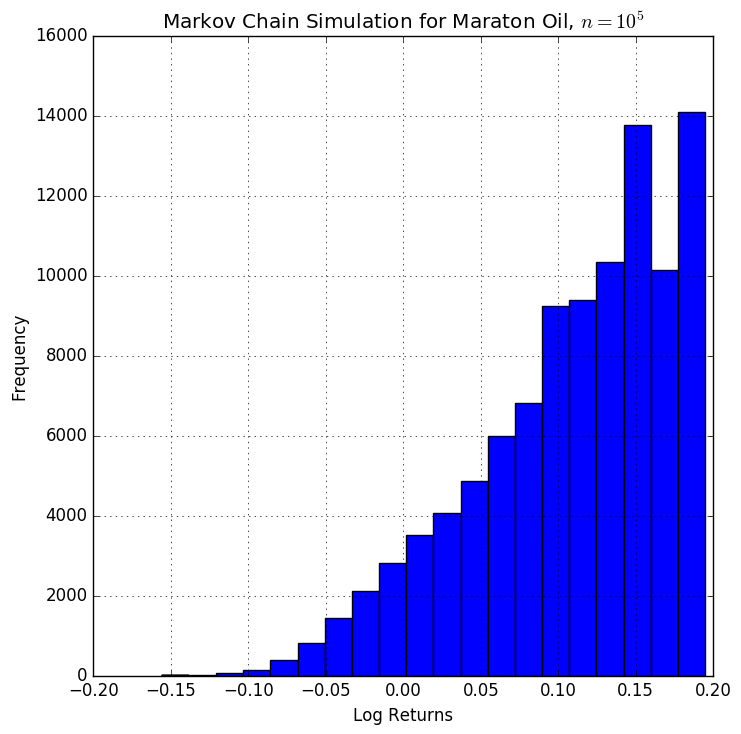
\includegraphics[width=0.85\textwidth]{mcLogReturns_5.png} 
\centering
\end{figure}


For $n = \{10^3, 10^4, 10^6\}$ see the Annex. 



\subsection{Second and N-order Markov Processes}
A second order, third order up to $\text{n}^{th}$ order Markov process behaves the same as described by \ref{smc}, except:
\begin{equation*}
Pr\left(X_t = x_i |X_{t-1},X_{t-2},...,X_{1}  \right) = Pr\left( X_t=x_i \right|X_{t-1}=x_{t-1},...,X_{t-n}=x_{t-n})
\end{equation*}

Given observable outcomes, choosing a model is a trade-off between a parsimonious model and a better goodness of fit. Given a likelihood function of the model $\mathbf{\Lambda}$, once can use a loss function, maximize a probability distribution or use AIC, e.i. $2k-\ln{\mathbf{\Lambda}}$. Another favourable characteristic of the N-order Markov Processes to be useful in practice is that the transition probability matrix $\mathbb{A}$ be \textbf{\textit{irreducible}}.

\begin{theorem}
Any N-order Markovian Process can be represented by a first order Markovian process. 
\end{theorem}
\begin{proof}
This is rather a trivial proof. Suppose we observe a process that is indeed governed by the function $f(x,y) \to \mathbb{R}$ where $x$, $y$ $\in$  state spaces $S,V$ respectively and we want to transform $f(x,y)$ into $f(z)$. We can define a state space $z \in$ $T = \{(x_i,y_j), \quad x_i \in S \quad y_j \in V  \}$ and then rewrite $f(x,y)$ as $f(z)$. 
\end{proof}
Of course the proof goes beyond saying that we can represent any 2-nd order Markov Chains, e.i.:
\begin{equation*}
Pr\left(X_t |X_{t-1},X_{t-2},...,X_{1}  \right) = Pr\left( X_t=x_i |X_{t-1}=x_{t-1},X_{t-2}=x_{t-2} \right)
\end{equation*}
as:
\begin{equation*}
Pr\left(X_t |X_{t-1},X_{t-2},...,X_{1}  \right) = Pr\left( X_t=x_i |(X_{t-1},X_{t-2}) \right)
\end{equation*}
where $(X_{t-1},X_{t-2})$ is defined as a new state. 
What the second fundamental theorem of Markov Chains suggests is that even if we have a very complex dynamic process which emits observations $\epsilon_i$, we can still describe it by a first order Markov chain, given enough states. 

\subsection{Semi Markov Chains and Semi Hidden Markov Models}
The SMC and the SHMM are a generalization of the MC and HMM in the sense that they:
\begin{enumerate}
\item Allow arbitrarily distributed sojourn times in any state
\item Still have the Markovian hypothesis, but in a more flexible manner.
\end{enumerate}
As defined by \cite{barbu08}[pp. 2] a process that has these two properties will be called a semi-Markov process.


\subsection{Continuous State Markov Chains}
A continuous state Markov Chain extends the model presented in section \ref{smc} by allowing a probability density distribution on the states. These have been analysed extensively in the paper of \cite{benesch2001baum}. 
More formally, a stochastic kernel on $\mathbb{S}$ is a function $p:\mathbb{S}\times \mathbb{S}\in \mathbb{R}$ with the property that:
\begin{align*}
 & p(x, y) \geq 0 \quad \forall x,y \in \mathbb{S} \\ 
 & \int_{-\infty}^{+\infty} p(x, y) dy = 1 \quad\forall x \in \mathbb{S}
\end{align*}

For example, suppose the random variable $X_t$ is characterized by the famous normally distributed random walk:
\begin{equation}\label{eq:RWalkNorm}
X_{t+1} = X_t + \xi_{t+1} \quad \text{where} \quad
\{ \xi_t \} \stackrel {\textrm{ IID }} {\sim} N(0, 1)
\end{equation}

We could characterize this random distribution through the use of a continuous state Markov Chain, specifically by defining the transition probability $p(x_t, x_{t+1})$ analogous to $\mathbb{A}$\footnote{also called stochastic kernel in literature, see for example http://quant-econ.net/jl/stationary\_densities.html} to be:
\begin{equation}
p(x_t, x_{t+1}) = \frac{1}{\sqrt{2 \pi}} \exp \left\{ - \frac{(x_{t+1} - x_t)^2}{2} \right\}
\end{equation}

Combining the ideas from the blog of \cite{quantecon} as well as the seminal paper \cite{Tauchen86} we can connect Stochastic difference equations to the probability kernel.
\begin{equation}\label{eq:genericKernel}
X_{t+1} = \mu(X_t) +\sigma(X_t)\xi_{t+1}
\end{equation}
where $\{ \xi_t \} \stackrel {\textrm{ IID }} {\sim} \phi$ and $\mu, \sigma$ are functions.
This is clearly a Markov process, since the state of the system at $t+1$ depends only on the current state $t$. 
Under this equation, which we will call \emph{generic Markov process}, we can write the normally distributed random walk stochastic process, as shown in \ref{eq:RWalkNorm} as a special case of equation \ref{eq:genericKernel} when $\sigma(x_t)=1$ and $\mu(x_t)=x_t$.

Consider  $X_t$ following an ARCH(1) process:
\begin{align*}
& y_{t}   = a_0 + a_1y_{t-1}+ a_2y_{t-2}+...+a_qy_{t-q-1} + X_t \\
& y_{t+1} = a_0 + a_1y_{t}+ a_2y_{t-1}+...+a_qy_{t-q} + X_{t+1} \\
& X_{t+1} = \alpha X_{t} + \sigma_t \xi_{t+1} \\
& \sigma_t^2 = \beta + \gamma X_t^2, \quad \text{where} \beta, \gamma >0
\end{align*}

This is a special case of equation \ref{eq:genericKernel} with $\sigma(x) = (\beta + \gamma x^2)^{1/2}$ and $\mu(x) = \alpha x$

Moreover, it is useful to write equation \ref{eq:genericKernel} in a form of a probability kernel. 
\begin{theorem}
Any Markov Process in the form $X_{t+1} = \mu(X_t) +\sigma(X_t)\xi_{t+1}$ as specified in equation \ref{eq:genericKernel} where $\xi_{t+1} \sim \phi$ can be written as:
\begin{equation}
Pr(x_{t+1}|x_t)
= \frac{1}{\sigma(x_t)}
\phi \left( \frac{x_{t+1} - \mu(x)}{\sigma(x)} \right)
\end{equation}
\end{theorem}
\begin{proof}
Let $U$ and $V$ be two random variables with probability density functions $f_U(u)$ and $f_V(v)$ and the cumulative probability distributions  $F_U$ and $F_V$ respectively and $V = a+bU$ where $a,b \in \mathbb{R}$ and $b>0$. Theorem 8.1.3 from \cite{quantecon} proves that in this case:
$f_V(v)= \frac{1}{b} f_U \left( \frac{v - a}{b} \right)$
and since $\sigma(x)$ is the square root of $\sigma^2(x)$ results that $\sigma(x)>0$ and we can apply Theorem 8.1.3 directly in our case which completes the proof. 
Proving theorem 8.1.3 from \cite{quantecon} is also straightforward:
We know that $F_V(v) = \mathbb P\{V \leq v \}$, and from the assumption that $V = a+bU$ we substitute $V$ and obtain  $F_V(v) = \mathbb P \{ a + b U \leq v \} = \mathbb P \{ U \leq (v - a) / b \}$. We can now write that:
\begin{equation}
F_V(v) = F_U ( (v - a)/b )
\end{equation}
and since the probability density function $f_V(v)$ is the derivative of the cumulative probability distribution $F_V(v)$ with respect to $v$, we take the derivative of $F_V(v)$ and obtain:
\begin{equation}
f_V(v)
= \frac{1}{b}
f_U \left( \frac{v - a}{b} \right)
\end{equation}
\end{proof}

For example, following the Solow-Swan model\footnote{In a nutshell, the Solow–Swan model assumes a closed market economy. A single good (output) is produced using two factors of production, labour $L$ and capital $K$ in an aggregate production function that satisfies the Inada conditions, which imply that the elasticity of substitution must be asymptotically equal to one. https://en.wikipedia.org/wiki/Solow-Swan\_model} presented in \cite{Romer06} the capital per capita $k$ difference equation is:
\begin{equation}\label{eq:SolowK}
k_{t+1} = s  A_{t+1} f(k_t) + (1 - \delta) k_t
\end{equation}
where 
\begin{enumerate}
\item $s$ is the savings ratio
\item $\delta$ is the normal depreciation rate of the capital
\item $A_{t+1}$ is the production shock at time $t+1$ which is latent at time $t$
\item and $f \colon \mathbb R_+ \to \mathbb R_+$ is a production function, usually of the labour augmenting Cobb-Douglas form.
\end{enumerate} 
Equation \ref{eq:SolowK} is the driving force of the most popular economic growth model in Economics.\footnote{Robert Solow has was awarder the Nobel Prize in Economics.} 
Since in equation \ref{eq:SolowK} the production shock $A_{t+1}$ is a random variable, it is also a special case of equation \ref{eq:genericKernel} with $\mu (x) = (1-\delta)x$ and $\sigma (x) = sf(x)$. Now we can also write the probability kernel of equation \ref{eq:SolowK} as:
\begin{equation}
p(x, y) = \frac{1}{sf(x)} \phi \left( \frac{y - (1 - \delta) x}{s f(x)} \right)
\end{equation} 
where $\phi \sim A_{t+1}$, $x = k_t$ and $y=k_{t+1}$.

Having defined the continuous probability transition density, we can generalize the formula for the probability state density at $t+1$.  In the continuous case, if the distribution of $X_t \sim \psi_t$ then $\psi_{t+1}$, analogous to the sum as specified in section \ref{smc} for the discrete case:
\begin{equation}\label{eq:CSMC_probVec}
\psi_{t+1}(y) = \int p(x,y) \psi_t(x) \, dx,
\qquad \forall y \in S
\end{equation}

\subsubsection{Simulating a Continuous State Markov Chain}
Once we have established a probability kernel and having the initial probability state distribution $\psi_0$, we can proceed to estimating the state density distribution $\psi_1$ at $t=1$. The straight forward way for simulating the growth of capital as described in equation \ref{eq:SolowK}: $k_{t+1} = s  A_{t+1} f(k_t) + (1 - \delta) k_t$ is to:

\begin{enumerate}
\item draw ${k_0}$ from the initial probability density $\psi_0$
\item draw $n$ parameters from the probability density $\phi$, in the case of the model at equation \ref{eq:SolowK} these are the technology shocks $A_1 ... A_n$. 
\item  repeat by computing $k_{t+1}$ from \ref{eq:SolowK} and store them in an array.
\end{enumerate}  
Once we have $n$ instances of $k_{t+1}$s, we can use kernel density estimates functions to make inferences about the probability distribution.\footnote{For example the open source library KernelDensity for Julia programming language which is hosted at https://github.com/JuliaStats/KernelDensity.jl} 

The paper of \cite{Stachurski2008}, based on the look-ahead estimator, provides an improved Monte Carlo algorithm for computing marginal and stationary densities of stochastic models with the Markov property, establishing global asymptotic normality and fast convergence. The idea is that, by the strong law of large numbers:
\begin{equation}
\frac{1}{n} \sum_{i=1}^n p(k_{t-1}^i, y)
\to
\mathbb E p(k_{t-1}^i, y)
= \int p(x, y) \psi_{t-1}(x) \, dx
= \psi_t(y)
\end{equation}
where $p(x,y)$ is the example specific stochastic kernel e.i. $p(x, y) = \frac{1}{sf(x)} \phi \left( \frac{y - (1 - \delta) x}{s f(x)} \right)$ 

Therefore, we can write our continuous state probability density as the average of probabilities:
\begin{equation}
\psi_t^n(y) = \frac{1}{n} \sum_{i=1}^n p(k_{t-1}^i, y)
\end{equation}

Since an efficient implementation of the Monte Carlo simulation for the continuous state Markov process requires a more significant number of steps than in the discrete case, as shown in section \ref{sec:SimMC}, and also taking into account that the continuous case is not conceptually different than in the discrete case, providing a step by step implementation as in section \nameref{sec:SimMC} is beyond the scope of this thesis. On the other hand,  I will present the implementation of \cite{Stachurski2008} in Julia language in the Annex for convenience purposes. 

Given the Solow-Swan model, and using the implementation of the \texttt{LAE, lae\_est} as provided in the Annex, we can now ask how fast does the initial density probability function for the continuous state Markov Chain converge to the steady state distribution of capital per capita $k$. To answer this question we only need to write the function for the probability kernel $p(x,y)$.

\begin{lstlisting}
function p(x, y)
    #=
    Stochastic kernel for the growth model with Cobb-Douglas production.
    Both x and y must be strictly positive.
    =#
    d = s * x.^alpha
    pdf_arg = clamp((y .- (1-sigma) .* x) ./ d, eps(), Inf) 
    return pdf(phi, pdf_arg) ./ d
end
\end{lstlisting}

The idea is that any initial state density distribution for the $k_0$ will converge to a steady state density distribution. 
Suppose the initial density distribution follows:
\begin{equation}
f(x; \alpha, \beta) = \frac{1}{B(\alpha, \beta)}
 x^{\alpha - 1} (1 - x)^{\beta - 1}, \quad x \in [0, 1]
\end{equation}
which is known as the Beta Distribution. 

\begin{lstlisting}
a_sigma = 0.4
phi = LogNormal(0.0, a_sigma) #Technological Change Distribution
psi_0 = Beta(1.8, 2.8) 
ygrid = linspace(0.01, 4.0, 200)
\end{lstlisting}

\begin{lstlisting}
fig, ax = subplots()
#for (x,y) in zip(ygrid, ygrid)
ax[:plot](ygrid, pdf(psi_0, ygrid), color="0.5")
t=LaTeXString(" Initial density Distribution: Beta(1.8,2.8) ")
ax[:set_title](t)
show()
\end{lstlisting}

We can plot the initial distribution of $\psi_0$
\begin{figure}[h]
\caption{Beta Distribution}
\label{fig:BD}
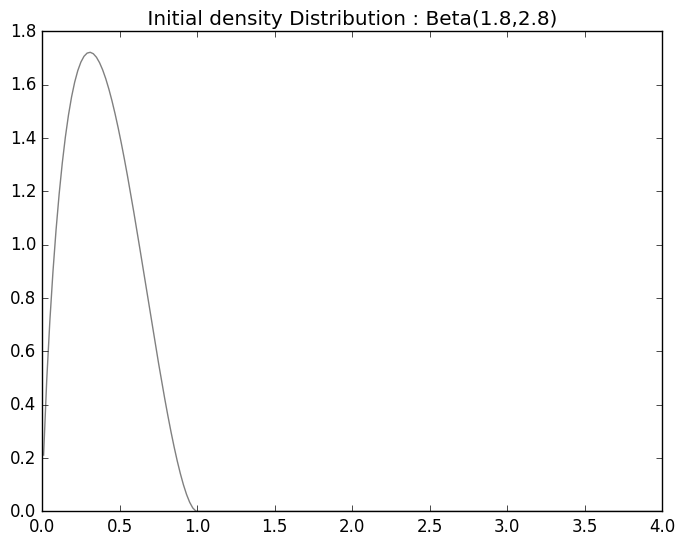
\includegraphics[width=0.95\textwidth]{BetaDistribution.png} 
\centering
\end{figure}
and then by iteratively applying the lae function with the density kernel, we can observe the speed of convergence.

\begin{lstlisting}
s = 0.2 # Savings Rate
\delta = 0.1 # Capital Depreciation Rate
a_\sigma = 0.4  # A = exp(B) where B ~ N(0, a_sigma)
\alpha = 0.4  # We set f(k) = k**alpha
\psi_0 = Beta(1.8, 2.8)  # Initial Continuous State distribution
\phi = LogNormal(0.0, a_\sigma)


n = 10000  # Number of observations at each date t
T = 30  # Compute density of k_t at 1,...,T+1

# Generate matrix s.t. t-th column is n observations of k_t
k = Array(Float64, n, T)
A = rand!(\phi, Array(Float64, n, T))

# Draw first column from initial distribution
k[:, 1] = rand(\psi_0, n)   # divide by 2 to match scale=0.5 in py version
for t=1:T-1
    k[:, t+1] = s*A[:, t] .* k[:, t].^\alpha + (1-\delta) .* k[:, t]
end
\end{lstlisting}

\begin{figure}[h]
\caption{Look Ahead Estimate}
\label{fig:LAEConvergence1}
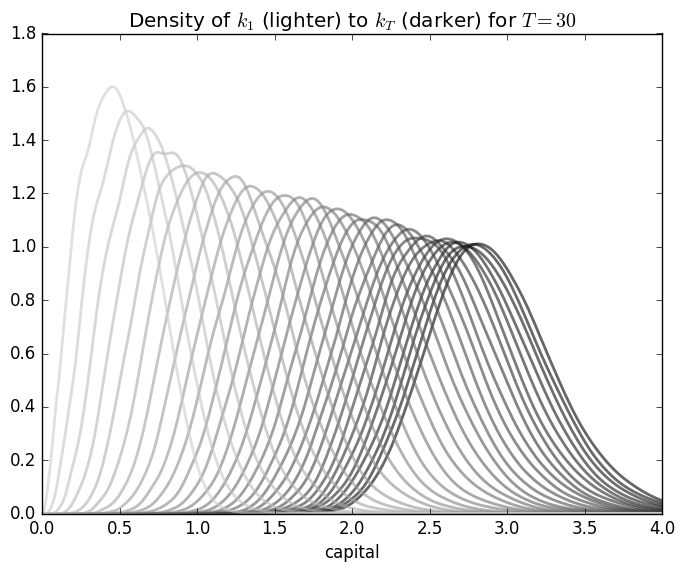
\includegraphics[width=0.95\textwidth]{CMCConvergence1.png} 
\centering
\end{figure}

Now let us take a more sophisticated probability distribution and observe the convergence. Suppose the initial continuous state distribution follows:
\begin{equation}
\begin{split}f(x; \xi, \sigma, \mu) = \begin{cases}
        \frac{1}{\sigma} \left[ 1+\left(\frac{x-\mu}{\sigma}\right)\xi\right]^{-1/\xi-1} \exp\left\{-\left[ 1+ \left(\frac{x-\mu}{\sigma}\right)\xi\right]^{-1/\xi} \right\} & \text{for } \xi \neq 0 \\
        \frac{1}{\sigma} \exp\left\{-\frac{x-\mu}{\sigma}\right\} \exp\left\{-\exp\left[-\frac{x-\mu}{\sigma}\right]\right\} & \text{for } \xi = 0
    \end{cases}\end{split}
\end{equation}
for
\begin{equation}
\begin{split}x \in \begin{cases}
        \left[ \mu - \frac{\sigma}{\xi}, + \infty \right) & \text{for } \xi > 0 \\
        \left( - \infty, + \infty \right) & \text{for } \xi = 0 \\
        \left( - \infty, \mu - \frac{\sigma}{\xi} \right] & \text{for } \xi < 0
    \end{cases}\end{split}
\end{equation}
known in the literature as the Generalized extreme value distribution. Unfortunately, this distribution throws an error. 

When trying to test the pareto distribution:
\begin{equation}
f(x; \alpha, \theta) = \frac{\alpha \theta^\alpha}{x^{\alpha + 1}}, \quad x \ge \theta
\end{equation}
with parameters (3,2), Julia kernel dies.

I have not enough information for the reasons why not all initial distributions converge. I have not tested whether restricting the range will solve this problem or whether there is a bug in the implementations of the distributions. 

On the other hand, the most popular distributions do work. For example the Levy distribution.
\begin{equation}
\begin{split}f(x; \mu, \sigma) = \sqrt{\frac{\sigma}{2 \pi (x - \mu)^3}}
\exp \left( - \frac{\sigma}{2 (x - \mu)} \right), \quad x > \mu\end{split}
\end{equation}

\begin{figure}[h]
\caption{Levy Distribution}
\label{fig:Levy Distribution}
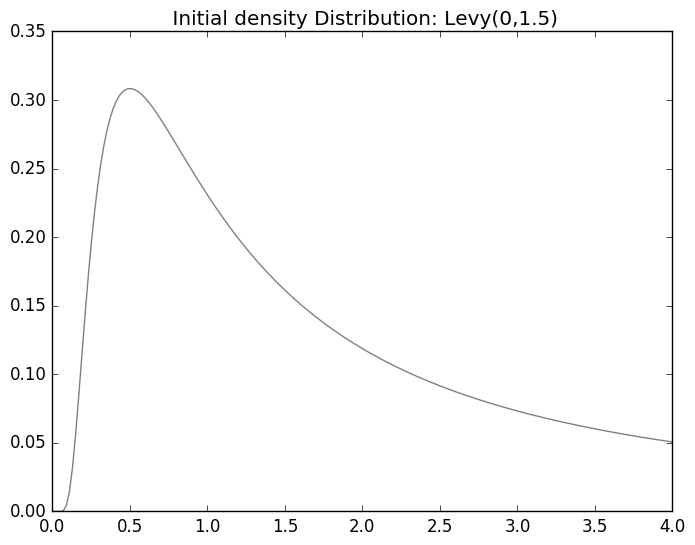
\includegraphics[width=0.95\textwidth]{LevyDist.png} 
\centering
\end{figure}

after 30 iterations of look ahead estimate with the same parameters as before:

\begin{figure}[h]
\caption{Levy Distribution Convergence}
\label{fig:LevyDistConvergence}
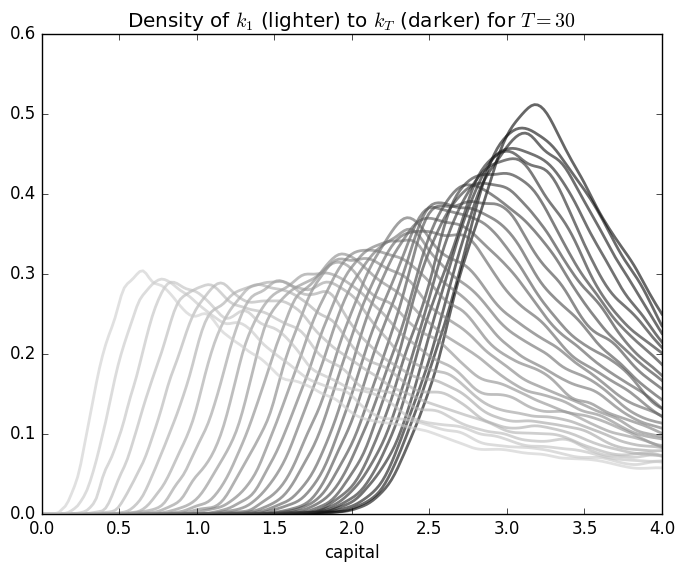
\includegraphics[width=0.95\textwidth]{LevyConvergence.png} 
\centering
\end{figure}


\begin{lstlisting}
s = 0.2 # Savings Rate
\delta = 0.1 # Capital Depreciation Rate
a_\sigma = 0.4  # A = exp(B) where B ~ N(0, a_sigma)
\alpha = 0.4  # We set f(k) = k**alpha
\psi_0 = Levy(0,1.5) # Initial Continuous State distribution
\phi = LogNormal(0.0, a_\sigma)
\end{lstlisting}


The conclusion about Continuous State Markov chains is that they are powerful tools to expend point estimates of economic aggregates. As we can see in our example, not only that capital per capita can have a wide range as a function of modest technology shocks, we cannot expect that with time the variance of our distribution will decrease as $t \to \infty$. In the case of the Levy distribution, we can see that the range the capital per effective capita, as seen in figure \ref{fig:LevyDistConvergence} can increase. 



\newpage
\section{The Hidden Markov Model and Latent Parameters Estimation}\label{HMM}
A great introduction into the workings of the Hidden Markov processes was presented by \cite{Rabiner89}. In a nutshell, a HMM is defined by a stochastic matrix $\mathbb{A}$ that changes the the states $s_i$ of the system according to some probability, where $s_i \in S$ and $S$ is the set of all possible States. These states are not observable. Each state can emit some observable outcomes with its own probability distribution which we will summarize in the emission matrix $\mathbb{B}$. We will take the example given by \cite[pp.9]{fraser08}.

\begin{figure}[h]
\caption{Hidden Markov Model from \cite[pp.9]{fraser08}}
\label{fig:HMM}
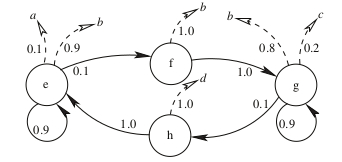
\includegraphics[width=0.85\textwidth]{HMM} 
\centering
\end{figure}

As we can see in figure \ref{fig:HMM}, we have an oriented graph which can easily be transposed to a HMM model. 

\[ \mathbb{A} = \begin{array}{c} e \\ f \\ g \\ h \end{array} \left( \begin{array}{cccc}
0.9 & 0.1& 0  & 0 \\
0   & 0  & 1  & 0 \\
0   & 0  & 0.9& 0.1 \\
1   & 0  & 0  & 0 \end{array} \right)\]

The emission probabilities for the events $\Sigma = \{a,b,c,d\}$, as specified in the \ref{smc}:
\[ \mathbb{B} = 
\begin{array}{c} e \\ f \\ g \\ h \end{array}
\begin{pmatrix} 
0.1 & 0.9 & 0 & 0 \\
0   & 1   & 0 & 0 \\
0 & 0.8 & 0.2 & 0 \\
0 & 0& 0& 1
\end{pmatrix} \]

Lastly, to fully define a HMM, we would either need a starting point, or an initial probability distribution among the states usually denoted by $\pi$. 

Having defined a hidden Markov model, we can endeavour to find answers to the following questions:
\begin{enumerate}
\item When was the last recession?
\item Are we still in the recession?
\item  What is the probability for the economy to follow a particular path of states?
\item What is the unconditional probability of observing certain outcome $e_i $ or what is the probability of being in a particular state $s_i$ e $Pr(S=s_i | e_i)$?
\end{enumerate}

We conclude that a Hidden Markov Model extends the class of the Markov Chain models, since any order of a Markov model can be represented as an HMM. 
We will denote a Hidden Markov Model by $\lambda(\mathbb{A},\mathbb{B},\pi)$.
\subsection{Simulating a Hidden Markov Model}
In this example we will generate a sequence of a balanced and an unbalanced coin that follows an HMM ($\lambda(\mathbb{A}, \mathbb{B}, \pi)$) in the Python programming language using the ghmm package. For installing the ghmm library please refer to the Annex and \href{http://ghmm.org}{http://ghmm.org}. 
\begin{equation}
\mathbb{A}= \left(\begin{array}{cc}
0.9 & 0.1 \\
0.2 & 0.8 \\
\end{array}\right)
\end{equation}

\begin{lstlisting}
import ghmm
A = [[0.9, 0.1], [0.2, 0.8]]
efair = [1.0 / 2] * 2
eloaded = [0.15, 0.85]
sigma = ghmm.IntegerRange(0,2)
B = [efair, eloaded]
pi = [0.5]*2
m = ghmm.HMMFromMatrices(sigma, ghmm.DiscreteDistribution(sigma), A, B, pi)
\end{lstlisting}
invoking the print method for the HMM model $m$
\begin{lstlisting}
print m

DiscreteEmissionHMM(N=2, M=2)
  state 0 (initial=0.50)
    Emissions: 0.50, 0.50
    Transitions: ->0 (0.90), ->1 (0.10)
  state 1 (initial=0.50)
    Emissions: 0.15, 0.85
    Transitions: ->0 (0.20), ->1 (0.80)
\end{lstlisting}
generating a sample of 40 observations and printing them.
\begin{lstlisting}
obs_seq = m.sampleSingle(40)
obs = map(sigma.external, obs_seq)

print obs

[1, 1, 0, 0, 1, 1, 1, 1, 1, 1, 1, 0, 0, 1, 1, 0, 1, 0, 0, 1, 0, 1, 0, 1, 0, 0, 0, 0, 0, 0, 1, 0, 1, 0, 0, 1, 1, 0, 1, 0]
\end{lstlisting}

For a dice simulation generated by an HMM, refer to appendix \ref{app:simHMM}.




\subsection{A formal introduction to an HMM}
Suppose we have identified a sequence $\mathcal{O} \in \mathbf{\Omega}$ that we assume is generated by an HMM: $\lambda(\mathbb{A},\mathbb{B},\pi)$ as defined in chapter \ref{HMM}. 
Given $\lambda$, we would like to know:
$$Pr(\mathcal{O}|\lambda)=? $$

A direct approach is that given the parameters of the HMM, we can compute the probability of observing a particular observation on a given chain of states:
\begin{equation}\label{eq:basic}
Pr\left(o_1,o_2,...,o_{T} |x_1,x_2,...,x_k,...x_T, \lambda \right)=  \pi_i b_i(o_1) \prod_{t=2}^{t=T} a_{t-1,t}b_{a_t}(o_t)
\end{equation}

And then we could sum the probabilities from equation \ref{eq:basic} over all possible states $X$:

\begin{equation}\label{eq:directApproach}
Pr\left(\mathcal{O} | \lambda \right)= \sum_X  \pi_i b_i(o_1) \prod_{t=2}^{t=T} a_{t-1,t}b_{a_t}(o_t) Pr(X|\lambda)
\end{equation}

Therefore, the direct approach is very difficult to assess. The difficulty of this problem consists in the fact that the total number of possibilities of sequences of states that can generate $\mathcal{O}$ is exponential in the number of observations $T$ and would require $\mathbf{\mathcal{O}}(N^T)$ operations, where $N$ is the total number of states. At a first glance this might not appear to be a particular big issue in Economics: consider analysing yearly aggregates of a span of 10 years with 2 states $\Omega = \{Recession, Growth\}$. If, however, we would increase the number of states to 3 and use quarterly data, finding the maximum would require years of computation - clearly not feasible for any practical purpose.\footnote{For a 2 state economy over a span of 10 years, we would call our function 1024 times, in contrast, a 3 state economy on quarterly data would require 12157665459056928801 ($1.22*10^{19}$) calls.} A better approach to calculate the unconditional probability $Pr(\mathcal{O}|\lambda)$ is the forward/backward algorithm which is a class of dynamic programming algorithms and takes advantage of the assumptions of the Markovian processes to filter all possible combinations of states $X$.

Secondly, another question of interest is to find the most likely sequence of states from $X$ given $\mathcal{O}$, e.i. the states that generated the highest probability $Pr(\mathcal{O}| X, \lambda)$.

Finally, the question that sparked my interest in studying Markovian processes is how do we estimate the parameters of an HMM, in particular $\mathbb{A}$ and $\mathbb{B}$. Unfortunately, this is still an unsolved problem in Mathematics and requires numerical methods. Once the matrix $\mathbb{A}$ is determined we can use the dynamic programming and combinatorial methods proposed by \cite{Lozovanu15} for determining the state-time probabilities and the matrix of limiting probabilities. These methods can be directly applied to refine not only the point estimates of long-term economic growth at the country level, as defined by the International Monetary Fond, but also update the concept of long term growth as an integral part of limiting probabilities of a HMM. 

To summarize, we could enumerate the key issues we would have to address and solve efficiently for an HMM model to be useful in practice. As expressed by \cite{fraser08} and \cite{hamilton02}: 

\begin{enumerate}
\item{Evaluation} - e.i. find the probability of an observed sequence given an HMM (relatively easy to do in practice)
\item{Decoding} - find the sequence of Hidden States that most likely generated the observation. That is: find the highest probability of a sequence. (until the Viterbi algorithm it was possible only theoretically)
\item{Learning} - Generate the best possible HMM for the observed outcome (really difficult - there are no analytic solutions to this problem. Use Baum-Welch algorithm)

\end{enumerate}



\subsection{The Forward/Backward Algorithm}\label{sec:FBA}
Given an HMM$(\mathbb{A}, \mathbb{B}, \pi)$, as introduced in section \ref{HMM} which we will denote by $\lambda(\mathbb{A}, \mathbb{B}, \pi)$, where $\mathbb{A}$ is the state transition probability e.i. $a_{ij}=a[i][j]=Pr(x_{t+1}=j|x_t=i)$  and $\mathbb{B}$ is the emissions probability, e.i. $b_i(k) = Pr(o_t = k|x_t=i)$ \footnote{ usually denoted by $\varepsilon_i(k)$ in the literature}, and $\pi$ is the initial probability distribution of states at $t=1$, e.i. $\pi_i = Pr(x_1=i)$, where $i \in \{1..N\}$, the objective of the forward/backward algorithm is to compute the probability of being in a particular state $x_t$ at time $t$, given a sequence of observations $\mathcal{O}$ e.i.:
\[ Pr(x_k | \mathcal{O})= ? , k \in \{1..T \} \] 
We can use Bayesian rule\footnote{In the appendix I will present the Bayesian rules in probability} to write $Pr(x_k | \mathcal{O} , \mathbf{\lambda})$ as 

\begin{equation}\label{eq:fb1}
Pr(x_k | O, \mathbf{\lambda}) =  \frac{Pr(x_k, \mathcal{O} | \mathbf{\lambda})}{Pr(\mathcal{O}|\mathbf{\lambda})} = \frac{Pr(x_k,o_1,o_2,...o_k |\mathbf{\lambda} )*Pr(o_{k+1},...,o_T|x_k,o_1,...o_k,\mathbf{\lambda})}{Pr(\mathcal{O}|\mathbf{\lambda})}
\end{equation}

Using the Markovian property in the second half of \ref{eq:fb1}\footnote{Since the current outcome depends on the current state and not on past outcomes $Pr(o_k|x_k,o_{k-1},o_{k-2}...) =Pr(o_k|x_k) $. In practice, it is reasonable to assume that the expected outcome of a function (the growth of Economy) depends on the intrinsic values that define the system, rather than past outcomes. } :

\begin{equation}\label{eq:fb2}
Pr(x_k | \mathcal{O}, \mathbf{\lambda}) = \frac{Pr(x_k,o_1,o_2,...o_k |\mathbf{\lambda} ) Pr(o_{k+1},...,o_T|x_k,\mathbf{\lambda})}{Pr(\mathcal{O}|\mathbf{\lambda})}
\end{equation}

The first part in the numerator of equation \ref{eq:fb2}, $Pr (x_k,o_1,o_2,...o_k |\mathbf{\lambda} )$ is called the forward part and $Pr(o_{k+1},...,o_T|x_k,\mathbf{\lambda})$ the backward part. 

Once we can find an algorithm to compute the forward and the backward part, we can compute $Pr(x_k | O, \mathbf{\lambda})$ which enables us to answer the following questions: \footnote{Mathematicalmonk channel present a gentle introduction to HMM and builds intuition what types of questions we can answer https://www.youtube.com/watch?v=7zDARfKVm7s\&list=PLD0F06AA0D2E8FFBA}

\begin{enumerate}
\item The Probability of being in a transition: $Pr(x_k \not= x_{k-1}|\mathcal{O})$
\item Helps augment the numerical methods in estimating the parameters of $\lambda$
\item Make samples on $x_k|\mathcal{O}$
\end{enumerate}




\subsubsection{Forward Algorithm}\label{sec:fa}
Given an HMM as presented in section \ref{HMM}: $\lambda(\mathbb{A}, \mathbb{B}, \pi)$, where $\mathbb{A}$ is the state transition probability e.i. $a_{ij}=a[i][j]=Pr(x_{t+1}=j|x_t=i)$  and $\mathbb{B}$ is the emissions probability, e.i. $b_i(k) = Pr(o_t = k|x_t=i)$ \footnote{ usually denoted by $\varepsilon_i(k)$ in the literature}, and $\pi$ is the initial probability distribution of states at $t=1$, e.i. $\pi_i = Pr(x_1=i)$, the objective of the forward algorithm is to compute
\begin{equation}\label{eq:fwa}
\alpha_i(k)=\alpha\left( x_k=i \right) = Pr(o_1,o_2,...o_k,x_k | \lambda) \quad\quad o_k \in \mathcal{O}, k=\overline{1,T} 
\end{equation}\footnote{I follow the notation of: http://personal.ee.surrey.ac.uk/Personal/P.Jackson/tutorial/hmm\_tut2.pdf}


The forward algorithm is also known as the \textit{filtering} algorithm as it uses the available information up to the point of $o_k \in \mathcal{O}$. Again, computing $Pr(o_1,o_2,...o_k,x_k | \lambda)$ directly would require a computation time exponential on $T$ and would not be feasible for practical purposes. 
On the other hand, we can use the \textit{Law of Total Probability}\footnote{I used the steps of the algorithm from Wikipedia, https://en.wikipedia.org/wiki/Forward\_algorithm except that I corrected for mistakes. For example: Wiki says it uses chain rule, when they meant the law of total probability.} and the Markov property to express:

If $k=1$, from the definition of $\lambda$: $$\alpha(x_k) = \pi_{x_k}$$

else:

\begin{align}
\alpha_i\left( x_k \right) =& \sum_{x_{k-1}} Pr(o_1,o_2,...o_k,x_{k-1},x_k | \lambda) \\
= &\sum_{x_{k-1}} Pr(o_k | o_1,o_2,...o_{k-1},x_{k-1},x_k, \lambda)\times \\&Pr(x_k|o_1,o_2,...o_{k-1},x_{k-1},\lambda) Pr(o_1,o_2,...o_{k-1},x_{k-1}|\lambda)
\\ =& \sum_{x_{k-1}} Pr(o_k | x_k, \lambda)Pr(x_k|x_{k-1},\lambda) \alpha\left( x_{k-1} \right)
\\ =& \sum_{x_{k-1}} \mathbf{b}_{x_k}(o_k)  \mathbf{a}_{(k-1,k)}\alpha\left( x_{k-1} \right) 
\\ =& \mathbf{b}_{x_k}(o_k) \sum_{x_{k-1}} \mathbf{a}_{(k-1,k)}\alpha\left( x_{k-1} \right) , \quad x_{k-1}=\overline{1,N}, k=\overline{2,T}
\end{align}

Therefore, we can calculate the probability of observing a particular state $x$ at time $t$ with a cost of $\mathcal{O}(N^2T)$ operations using this recursive algorithm which is linear in $T$, rather than exponential for the naive approach. 

Once we have a procedure to efficiently calculate $\alpha_i(k)$ we can also express the unconditional probability of observing $\mathcal{O}$ as the sum of all $\alpha_i(T)$ over all states.
\begin{equation}\label{eq:Pr(O)}
Pr(\mathcal{O}|\lambda) = \sum_{i=1}^N \alpha_i(x_T)
\end{equation}

\subsubsection{Backward Algorithm}\label{sec:ba}
The backward algorithm is the second part of the forward/backward algorithm in equation \ref{eq:fb2}.

As in subsection \ref{sec:fa} we assume that an HMM as presented in section \ref{HMM}: $\lambda(\mathbb{A}, \mathbb{B}, \pi)$ is given, where $\mathbb{A}$ is the state transition probability and $\mathbb{B}$ is the emission probability matrix, e.i. $b_i(k) = Pr(o_t = k|x_t=i)$ and $\pi$ is the initial state probability distribution, the objective of the backward algorithm is to compute:
\begin{equation}\label{eq:ba1}
\beta_i(k)=\beta(x_k=i) = Pr(o_{k+1},o_{k+2},...,o_{T} | x_k=i, \lambda) \quad i=\overline{1,N}, k=\overline{1,T}
\end{equation}
Again, to get the recursive approach we will make use of the law of total probability to write:
\begin{align}
\beta(x_k) =&  Pr(o_{k+1},o_{k+2},...,o_{T} | x_k=i, \lambda) \\
=& \sum_{x_{k+1}} Pr(o_{k+1},o_{k+2},...,o_{T},x_{k+1} | x_k=i, \lambda)
\end{align}
Now we can divide se sequence of observables and isolate the $o_{k+1}$ observation as follows:
\begin{align}
\beta(x_k) =& \sum_{x_{k+1}} Pr(o_{k+2},...,o_{T}|x_{k+1},x_{k}=i,o_{k+1}, \lambda)\times\\
&Pr(o_{k+1}|x_{k+1},x_{k}=i,\lambda) \times Pr(x_{k+1}|x_{k}=i,\lambda) 
\end{align}
Now using the Markovian property and the fact that $Pr(o_{k+1}|x_{k+1},x_{k}=i,\lambda) = Pr(o_{k+1}|x_{k+1},\lambda)$

\begin{align}
\beta(x_k) &= \sum_{x_{k+1}}\beta(x_{k+1})\mathbf{b}_{k+1}(o_{k+1})\mathbf{a}_{k,k+1}, \quad\quad k=\overline{1,T-1}
\end{align}
The trick in the backward algorithm is that as shown above, $k$ takes values from $1$ to $T-1$. For $k=T$, we define:
$$\beta(x_T)=1$$ 
The intuition for this is clear when applying these algorithms to tagging problems in the Natural Language Programming, since we can define the state of the end of a sentence to be a special symbol "STOP". And since every sentence ends with this special symbol, the probability of getting $x_{T+1}=STOP$ equals $1$.


\subsection{The Viterbi Algorithm}
Given an HMM model $\lambda(\mathbb{A,B},\pi)$ and an observable sequence $\mathcal{O} = \{o_1,o_2,...,o_T \}$, we want to find the sequence $X=\{x_1,x_2,...,x_T\}$ that maximizes the probability in equation \ref{eq:basic}:

\begin{equation}
Pr\left(\mathcal{O}, x_1,x_2,...x_T,| \lambda \right)= \underset{X}{\operatorname{argmax}} \: \pi_i b_i(o_1) \prod_{t=2}^{t=T} a_{t-1,t}b_{a_t}(o_t)
\end{equation}

In a nutshell, the Viterbi algorithm examines at each step all the possibilities of getting to that particular state and retains only the most likely path to it, thus eliminating all other possibilities.\footnote{Simple as it may sound, according to David Forney }

For the first step, the probability of being in state $x_k$ at time $t=1$ and observing $o_1$ is simply an updated version of $\pi_k$.
$$Pr(x_1=k|o_1,\lambda) = \frac{Pr(x_1=k,o_1)}{\sum_{x_1\in S}Pr(x_1,o_1)}= \frac{\pi_{x_1}b_{x_1}(o_1)}{\sum_{x_i \in S} \pi_{x_i}b_{x_i}(o_1)}$$
where $s \in S$ and $S = \{1..N\}$ the set of all possible states. 
But we can still reduce the complexity of this formula by dropping the denominator, since maximizing the probability depends only on the numerator part, therefore:
\begin{equation}
V_{1,k}=\pi_{x_k}b_{x_k}(o_1)
\end{equation}
For the next iterations:
\begin{equation}
V_{t,k} = \underset{x_{t-1}\in S}{\operatorname{max}}\left( V_{t-1,x_{t-1}} \mathbf{a}_{x_{t-1},k} \mathbf{b}_{k}(o_t) \right)
\end{equation}
$$ \mathbf{V}_t = \{V_{t,k}|k \in  S\} $$
We denote the sequence of $X = \{ x_1,x_2,...,x_T \}$ that generates $V_T$:
$$\mathbf{x}_T = \underset{x\in S}{\operatorname{arg\, max}}\mathbf{V}_{T,x}$$
The algorithm's complexity is $\mathcal{O}(N^2*T)$ which is linear in T. 
\subsection{The EM algorithm}\label{sec:EM}
The Expectation Maximization algorithm was describe in the paper of \cite{Dempster77}. 
The Baum-Welch algorithm extends the class of the EM algorithm and so we will focus on Baum-Welch instead. 

\subsection{The Baum-Welch Algorithm}\label{sec:BW}
Given an observable sequence $\mathcal{O} = \{o_1,o_2,...,o_T \}$ and assuming this sequence was generated by an HMM model $\lambda(\mathbb{A,B},\pi)$ as define in section \ref{HMM}, we want to find out the most likely set of parameters of $\lambda$ that generated the sequence $\mathcal{O}$. Denoting by $\theta = \{\mathbb{A,B},\pi\}$ the set of parameters of $\lambda$, we want to find out $\theta$ that maximizes the probability: 

$$\theta^{\star} = \underset{\theta}{\operatorname{arg\, max}}Pr\left(\mathcal{O} | \lambda(\theta)\right)$$

The Baum-Welch algorithm uses as the basis the EM algorithm, which in turn is very similar to the k-means algorithm.  

The first step is to infer the number of states and initial parameters of the  $\lambda(\mathbb{A,B},\pi)$ using heuristic methods. 

Secondly, using the forward/backward algorithm as described in section \ref{sec:FBA} from page \pageref{sec:FBA} we find the updated Bayesian probability of observing $o_t$ at time $t$ in state $x_i$ :
\begin{equation}\label{eq:gamma}
Pr\left(x_t=i|\mathcal{O},\lambda(\theta)\right) =  \frac{\alpha_i(t) \beta_i(t)}{\sum_{j \in S}\alpha_j(t) \beta_j(t) }
\end{equation}
we will denote equation \ref{eq:gamma} by:
\begin{equation}
\gamma_i(t) = Pr\left(x_t=i|\mathcal{O},\lambda(\theta)\right)
\end{equation}
please note that in equation \ref{eq:gamma} the denominator $\sum_{j \in S}\alpha_j(t) \beta_j(t) $ was used rather that a computationally more efficient $\sum_{i \in S} \alpha_i(x_T) = Pr(\mathcal{O}|\lambda(\theta))$ in order to make $\gamma_i(t)$ a probability distribution.


Also, using the same backward and forward procedures as described in equation \ref{eq:ba1} and \ref{eq:fwa} we can also compute the probability of switching from state $x_k=i$ to $x_{k+1}=j$ given a particular model $\lambda(\theta)$:

\begin{equation}\label{eq:xi}
Pr(X_t=i,X_{t+1}=j|\mathcal{O},\lambda) = 
\frac{\alpha_i(t) a_{ij} b_j(o_{t+1}) \beta_j(t)}{Pr(\mathcal{O}|\lambda(\theta))}
\end{equation}
we will denote equation \ref{eq:xi} by
\begin{equation}
\xi_{ij}(t) = Pr(X_t=i,X_{t+1}=j|\mathcal{O},\lambda)
\end{equation}

Again, we need to make \ref{eq:xi} a probability distribution, and even though it looks computationally attractive to rewrite the denominator as the probability of observing $\mathcal{O}$ either by the forward or backward algorithm, we cannot write  \ref{eq:xi}, although wikipedia does\footnote{https://en.wikipedia.org/wiki/Baum-Welch\_algorithm}, as:
\begin{equation}
\xi_{ij}(t) =  
\frac{\alpha_i(t) a_{ij} b_j(o_{t+1}) \beta_j(t+1)}{\sum_{j\in S} \alpha_j(T)}
\end{equation}
for $\xi_{ij}(t)$ to be a probability distribution:
\begin{equation}
\xi_{ij}(t) =  \frac{\alpha_i(t) a_{ij} b_j(o_{t+1}) \beta_j(t+1)}
					{\sum_{i\in S}\sum_{j\in S} \alpha_i(t) a_{ij} b_j(o_{t+1}) \beta_j(t+1) }
\end{equation}

Now recall that $a_{ij}$ is the probability of moving to state $j$ while already being in state $i$, e.i. 
\begin{equation}
a_{ij}= Pr(x_{t+1}=j|x_t=i, \mathcal{O}, \lambda(\theta)
\end{equation}


We can rewrite the above equation of $a_{ij}$  by applying the Bayesian rule:
\begin{equation}\label{eq:aij}
Pr(x_{t+1}=j|x_t=i, \mathcal{O}, \lambda(\theta) = \frac{Pr(x_{t+1}=j,x_t=i| \mathcal{O}, \lambda(\theta)}{Pr(x_t=i | \mathcal{O}, \lambda(\theta)}
\end{equation}

Using equations \ref{eq:xi} and \ref{eq:gamma} in equation \ref{eq:aij} we can finally obtain the posterior distribution of $\bar{a_{ij}}$:

\begin{equation}
\bar{a_{ij}} = \frac{\sum_{t=1}^{T-1}\xi_{ij}(t)}{\sum_{t=1}^{T-1} \gamma_i(t)} 
\end{equation}
equivalently:
\begin{equation}
\bar{a_{ij}} = \dfrac{\dfrac{Pr(x_{t+1}=j,x_t=i| \mathcal{O}, \lambda(\theta)}{Pr(x_t=i | \mathcal{O}, \lambda(\theta)}}
		 {\dfrac{\alpha_i(t) \beta_i(t)}{\sum_{j \in S}\alpha_j(t) \beta_j(t) }}
\end{equation}
substituting 
\begin{equation}
\bar{a_{ij}} = \dfrac{  \dfrac{\alpha_i(t) a_{ij} b_j(o_{t+1}) \beta_j(t+1)}
					{\sum_{i\in S}\sum_{j\in S} \alpha_i(t) a_{ij} b_j(o_{t+1}) \beta_j(t+1) }}
					{\dfrac{\alpha_i(t) \beta_i(t)}{\sum_{j \in S}\alpha_j(t) \beta_j(t) }}
\end{equation}
now we have a formula for re-estimating the transition probabilities as a function of the backward and forward probabilities, both of which are linear in $T$. 

To update the initial state probability distribution: 
\begin{equation}
\bar{\pi_i} = \gamma_1(i) = \frac{\alpha_i(1)\beta_i(1)}{\sum_{i \in S} \alpha_i(1)\beta_i(1) }
\end{equation}

For the emissions probability we have the expected number of the system being in state $i$ and observing $o_k$ :
\begin{equation}
\bar{b_i(o_k)} = \frac{\sum_{t \in T} \gamma_t(i) \mathbf{1}_{o_t=o_k}}{\sum_{t \in T} \gamma_t(i)}
\end{equation}


Therefore, given a model $\lambda$ , we can compute $\bar{lambda}(\bar{\mathbb{A}}, \bar{\mathbb{B}}, \bar{\pi})$ and using the results of the theorem provided by \cite{baum1967}, specifically:
\begin{theorem}
Let $P(x) = P (\{x_{ij} \})$ be a polynomial with non-negative coefficients homogeneous of degree $d$. If $x_{ij} \geq 0$ and $\sum_j x_{ij}=1$. Denoting:
\begin{equation}
\mathfrak{I}(x)_{ij}= 
\dfrac{\left( x_{ij} \dfrac{\partial P}{\partial x_{ij}} \middle |_{(x)} \right)}
{\left( \sum_j x_{ij} \dfrac{\partial P}{\partial x_{ij}} \right)  }  
\end{equation}
then $\mathbb{P}(\mathfrak{I}(x_{ij})) \geq \mathbb{P}(x_{ij}) $
\end{theorem}
\begin{proof}
The proof is provided by \cite{baum1967}.
\end{proof}
we conclude that $\bar{\lambda}$ is a \textit{better} HMM model than $\lambda$. By \textit{•}{better} we mean that
\begin{equation}
\mathbb{P}(\mathcal{O}|\bar{\lambda} \geq \mathbb{P}(\mathcal{O}|\lambda)
\end{equation}
Therefore we have obtained an improved version of $\lambda$. Repeating this process iteratively we will converge to a local maximum. There is no guarantee however that this local maximum will also be a global maximum. Since the optimization surface of a Markov process can be extremely complex, what we can do is randomly assign initial probability distributions $\mu_i$ for $i \in \bar{1..n}$ and compare the local optima for each $i$, hoping we reached the highest value. Most importantly, these new estimated probabilities $\bar{A}, \bar{B}$ need to make sense, therefore the holistic and heuristic reviews of the most likely models $\lambda_i$ need to be performed by experts in the field. 

The implementation of the Baum Welch algorithm is at the heart of the open source HMM implementation\footnote{see: http://ghmm.org/}.

To show for convenience purposes how the Baum Welch algorithm works in practice, we will use the data from the example provided by \href{http://dna.cs.byu.edu/bio465/Labs/hmmtut.shtml}{byu.edu}\footnote{link: \href{http://dna.cs.byu.edu/bio465/Labs/hmmtut.shtml}{http://dna.cs.byu.edu/bio465/Labs/hmmtut.shtml}}, consider the nucleotide sequence $\{a, c, g, t\}$, assume there is an HMM model $\lambda(\mathbb{A,B},\pi)$ and the observations $\mathcal{O}$:

\begin{lstlisting}
['g', 'c', 'c', 'g', 'g', 'c', 'g', 'c', 'g', 'c', 'g', 'c', 'c', 'g', 'c', 'g', 'c', 'g', 'c', 'g', 'c', 'c', 'g', 'c', 'g', 'c', 'c', 'c','t', 't', 't', 't', 't', 't', 'a', 't', 'a', 'a', 'a', 'a', 't', 't', 't', 'a', 't', 'a', 't', 'a', 'a', 'a', 't', 'a', 't', 't', 't', 't','g', 'c', 'c', 'g', 'g', 'c', 'g', 'c', 'g', 'c', 'g', 'c', 'c', 'g', 'c', 'g', 'c', 'g', 'c', 'g', 'c', 'c', 'g', 'c', 'g', 'c', 'c', 'c','t', 't', 't', 't', 't', 't', 'a', 't', 'a', 'a', 'a', 'a', 't', 't', 't', 'a', 't', 'a', 't', 'a', 'a', 'a', 't', 'a', 't', 't', 't', 't']
\end{lstlisting}
generated by two states $normal, island$. We would like to know what was the sequence of states that generated these observations and would also like to see the most likelihood matrix $\mathbb{A}$ from the $\lambda$.

The software implementation is provided in the Annex \ref{app:simHMM}. 


As we see we have obtained $\bar{\lambda}$ with updated transition probabilities. 



\newpage
\section{Conclusions}
As we have seen in the first part of this thesis Markov Chains have a wide area of applicability in modelling topics in Economics and Finance. Moreover, they provide a fresh paradigm for viewing traditional concepts in Economics such as long term economic growth or stock returns in Finance. The extension of the discrete state Markov chain to continuous states allows us to see the dynamics of the very probability distribution of the variable of interest rather than point estimates. Also, we have seen that the initial distribution assumptions play a crucial role in the variance of subsequent distributions and most importantly, the dispersion not only remains persistent after long periods of time (30 cycles in our case) but it can also increase casting doubt about concepts such as long run equilibrium \textit{steady states}. On the other hand, Markov Chains are sensitive to how we define and what we incorporate in such abstract concepts as \textit{states}. Even if we assume that the economy is governed by distinct economic states, it is still a matter of opinion when deciding the number of states. Nevertheless, I avail myself to conclude that the advantages of augmenting a model even with a parsimonious 2 state Markov Model can be expected to yield significant improvements. 

A more general model of the Markov Chains that we have discussed in section \ref{HMM}, suitable with latent states or imperfect information, is the Hidden Markov Model (also called regime switching model in some sources). It not only allows better fit of traditional econometrics models such as ARMA and ARIMA, it does so using fewer parameters. The drawbacks of the HMM is its complexity and computational requirements in estimating the state transition probabilities. Fortunately, we have concluded that the use of dynamic programming techniques such as the Baum-Welch algorithm, extensively described in \ref{sec:BW} partially solves these problems. The drawback of the Baum-Welch algorithm is that it does not guarantee a global optimum but only a local one and depending on the model, many random iterations of the initial probability distributions are needed to find the parameters of the HMM that generated the observations. 

On future work I would like to continue on focusing on Hidden Markov Models and provide solutions to the problem of finding the global optimum. One way is to take advantage of computing parallelism or network distributed systems. This is possible since the bottleneck of estimating the transition probability matrix is in computing power and not in the network of the dimensions of the training set. Using mapreduce functions the central node can easily retain the highest likelihoods and discard others. Furthermore, I would like to further advance the HMM in the continuous state space and allow dimensionality reduction of external variables when defining abstract states of an HMM. 

On a more philosophical note, we can conclude that history doesn't matter for the future if we know \textit{the present}. Therefore, predicting future returns, especially growth rates, solely on past returns is the wrong path. But do we know \textit{the present}? 

\newpage
\appendix
\section{Replication}
All script files can be found at my GitHub repository at \href{https://github.com/moldovean/usm/tree/master/Thesis}{https://github.com/moldovean/}\footnote{\href{https://github.com/moldovean/usm/tree/master/Thesis}{https://github.com/moldovean/usm/tree/master/Thesis}}.
For any questions, please do not hesitate to contact me at \href{adrian@vrabie.net}{adrian@vrabie.net}
\subsection{Installing the GHMM library}
Unfortunately the GHMM cannot be installed using pip command, on the other hand, the installation instructions to build the GHMM package can be found at \href{http://ghmm.org}{http://ghmm.org} and are fairly easy. For convenience purposes I will list the terminal commands for Ubuntu (Debian Linux). 
First of all the ghmm package has some requirements:
\begin{lstlisting}
sudo apt-get update 
sudo apt-get install build-essential automake autoconf libtool
sudo apt-get install python-dev libxml++2.6-dev swig
\end{lstlisting}

Now create a new folder (ex. ghmm) and copy the source files from \href{http://sourceforge.net/svn/?group\_id=67094}{sourceforge}\footnote{link: \href{http://sourceforge.net/svn/?group\_id=67094}{http://sourceforge.net/svn/?group\_id=67094} }. Extract them in the newly created folder.  
Now we are ready to install the ghmm package for Python2.7+. 
\begin{lstlisting}
cd ghmm
sh autogen.sh
sudo ./configure
sudo make
sudo make install
sudo ldconfig
\end{lstlisting}
Check your installation. In Python:
\begin{lstlisting}
>> import ghmm
\end{lstlisting}


\section{Figures}

\begin{figure}[h]
\centering
\begin{subfigure}{.5\textwidth}
  \centering
  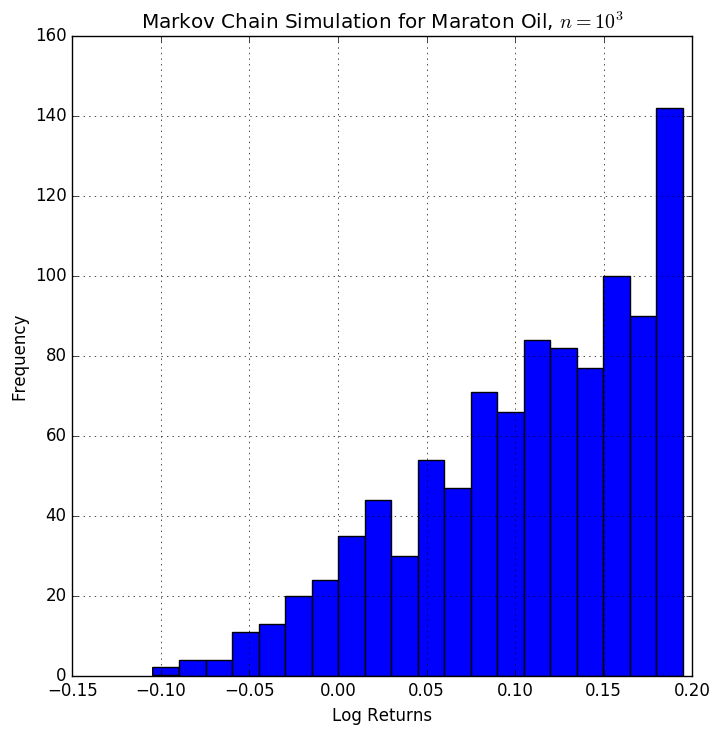
\includegraphics[width=0.95\textwidth]{mcLogReturns_3.png} 
  \caption{n=$10^3$}
  \label{fig:MCSim3}
\end{subfigure}%
\begin{subfigure}{.5\textwidth}
  \centering
  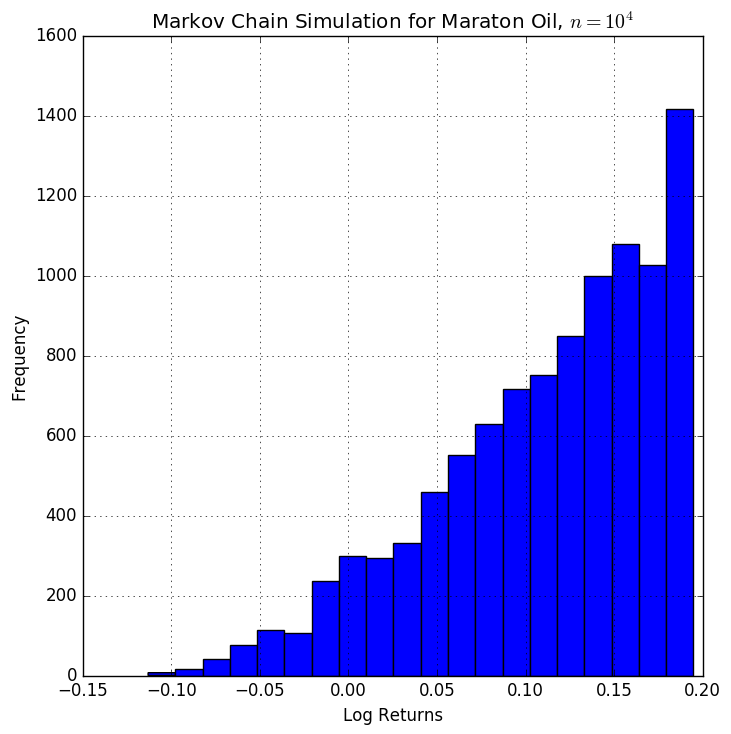
\includegraphics[width=0.95\textwidth]{mcLogReturns_4.png} 
  \caption{ n = $10^4$}
  \label{fig:MCSim4}
\end{subfigure}
\caption{Markov Chain Simulation}
\label{fig:DiscreteMCSim1}
\end{figure}

\begin{figure}[h]
\centering
\begin{subfigure}{.5\textwidth}
  \centering
  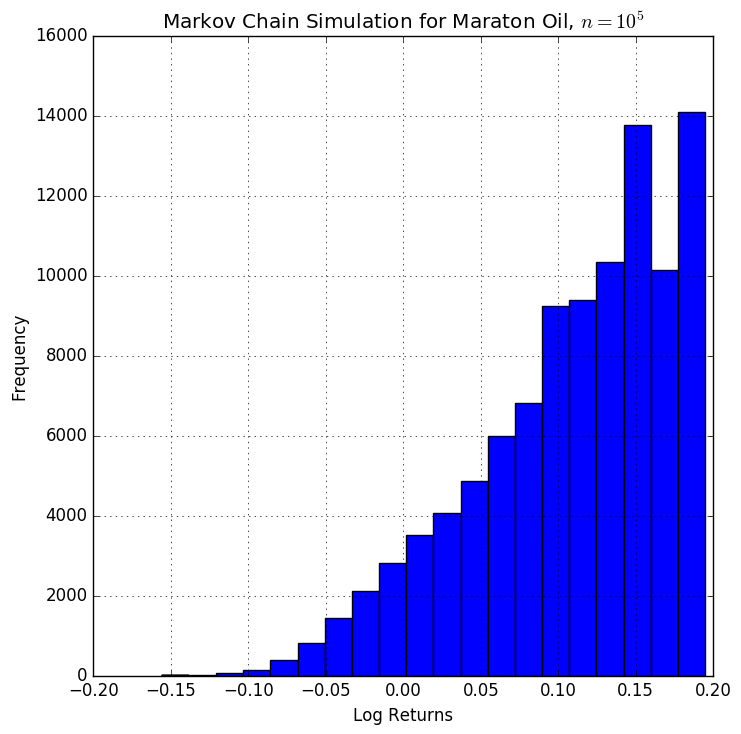
\includegraphics[width=0.95\textwidth]{mcLogReturns_5.png} 
  \caption{n=$10^5$}
  \label{fig:MCSim5_2}
\end{subfigure}%
\begin{subfigure}{.5\textwidth}
  \centering
  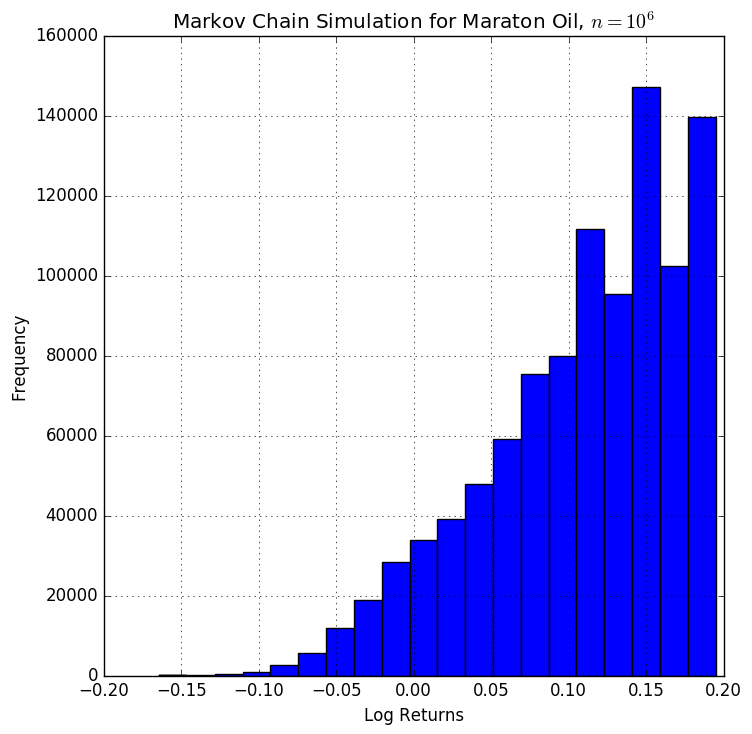
\includegraphics[width=0.95\textwidth]{mcLogReturns_6.png} 
  \caption{n=$10^6$}
  \label{fig:MCSim6}
\end{subfigure}
\caption{Markov Chain Simulation}
\label{fig:DiscreteMCSim2}
\end{figure}

As the simulation for the discrete state Markov Chain shows, the distribution of the returns stabilizes with $n=10^4$ simulations. Using these histograms we can apply non-parametric methods to obtain the KDE or use the frequency approach to answer decision-making related questions. For example: \textit{What is the probability that Maraton oil will lose money from investing in Kurdistan region of Iraq?}.

\section{Theoretical requirements}
\subsection{Bayesian Estimation}
Bayesian estimation is simply a rearrangement of the conditional probability formula.
\begin{equation}
\mathbb{P}(A|B) = \frac{\mathbb{P}(A,B)}{\mathbb{P}(B)} = \frac{\mathbb{P}(B|A)*\mathbb{P}(A)}{\mathbb{P}(B)}
\end{equation}
At the moment there is a dire lack of intuitive written books in probability and statistics, see for example \href{http://stats.stackexchange.com/questions/70545/looking-for-a-good-and-complete-probability-and-statistics-book}{stackexchange.com question}\footnote{link: http://stats.stackexchange.com/questions/70545/looking-for-a-good-and-complete-probability-and-statistics-book}
For more information about Bayesian rule and applications of Bayesian estimation on the parameters of a probability distribution, I recommend  \href{https://onlinecourses.science.psu.edu/stat414/node/241}{http://psu.edu/}\footnote{link: \href{https://onlinecourses.science.psu.edu/stat414/node/241}{https://onlinecourses.science.psu.edu/stat414/node/241}}. Some people recommend \href{https://www.statlect.com/fundamentals-of-probability/Bayes-rule}{http://www.statlect.com/}\footnote{link: https://www.statlect.com/fundamentals-of-probability/Bayes-rule} because they also provide accessible proofs of elementary and less elementary facts that are difficult to find in probability and statistics books. Another popular site for statistics is \href{http://stattrek.com/probability/bayes-theorem.aspx}{http://stattrek.com/}\footnote{link: http://stattrek.com/probability/bayes-theorem.aspx}
\subsection{Eigenvalues and Eigenvectors}
Let $A$ be an $n\times n$ matrix and $\mathbf{x}$ be an $n\times 1$ vector. If the product $A\mathbf{x}$ points in the same direction as the vector $\mathbf{x}$, then $\mathbf{x}$ is an eigenvector of $A$. Eigenvalues and eigenvectors describe what happens when a matrix is multiplied by a vector. For a rigorous introduction to eigenvalues and eigenvectors consider the open \href{http://ocw.mit.edu/courses/mathematics/18-06sc-linear-algebra-fall-2011/least-squares-determinants-and-eigenvalues/eigenvalues-and-eigenvectors/}{MIT course} \cite{MITLA}. 
For an interactive learning and building a sense of feel of what eigenvectors and eigenvalues are, consider \href{http://setosa.io/ev/eigenvectors-and-eigenvalues/}{http://setosa.io}\footnote{link: http://setosa.io/ev/eigenvectors-and-eigenvalues/} which uses the \href{http://threejs.org/}{http://threejs.org/} visualisation library. 

\section{Code Implementation}
\subsection{Look Ahead Estimate Implementation}
This code was implemented by  Spencer Lyon and referenced by \citep{Stachurski2008} in the \cite{quantecon} blog. It implements a class for the purpose of simulating a continuous state Markov process. The implementation leveraged on the paradigm of object oriented programming and creates a class \texttt{LAE} (Look Ahead Estimate) which takes the stochastic kernel $p$ and the observations vector $n \times 1$ vector.

\begin{lstlisting}
#=
Creats and Object which will be used to compute a sequence of marginal densities for a continuous state space Markov chain where the transition probabilities can be represented as densities rather than a discrete distribution. 
@author : Spencer Lyon <spencer.lyon@nyu.edu> @date: 2014-08-01
@modified: Adrian Vrabie <adrian@vrabie.net> @date: 2016-05-17
References: http://quant-econ.net/jl/stationary_densities.html
=#

"""
A look ahead estimator associated with a given stochastic kernel p and a vector
of observations X.

##### Fields
- `p::Function`: The stochastic kernel. Signature is `p(x, y)` and it should be
vectorized in both inputs
- `X::Matrix`: A vector containing observations. Note that this can be passed as
any kind of `AbstractArray` and will be coerced into an `n x 1` vector.

"""
type LAE
    p::Function
    X::Matrix

    function LAE(p::Function, X::AbstractArray)
        n = length(X)
        new(p, reshape(X, n, 1))
    end
end
\end{lstlisting}

The function \texttt{lae\_est} takes as input a \texttt{LAE} object and a vector or points $y$ which in our case represent quantities of capital. Then the function simply calculates the average of the probability kernel applied to these points $y$ and returns the average without dimensions (the \texttt{squeeze} function). 

\begin{lstlisting}

"""
A vectorized function that returns the value of the look ahead estimate at the
values in the array y.
##### Arguments
- `l::LAE`: Instance of `LAE` type
- `y::Array`: Array that becomes the `y` in `l.p(l.x, y)`
##### Returns
- `psi_vals::Vector`: Density at `(x, y)`
"""

function lae_est{T}(l::LAE, y::AbstractArray{T})
    k = length(y)
    v = l.p(l.X, reshape(y, 1, k))
    psi_vals = mean(v, 1)
    return squeeze(psi_vals, 1)
end
\end{lstlisting}


\subsection{Viterbi Algorithm}
The goal of this subsection is to create a parsimonious implementation of the Viterbi algorithm for demonstration purposes. I used the default Python 2.7 and IPython Notebook, but it should work in Python 3.+ as well, though I did not test it. 

\begin{lstlisting}

def viterbi(obs, states, start_p, trans_p, emit_p):
	//obs - Observations vector
	
    V = [{}]
    for s in states:
        V[0][s] = start_p[s]*emit_p[s][obs[0]]
    for t in range(1,len(obs)):
        V.append({})
        for s in states:
            V[t][s] = max(V[t-1][s_i]*trans_p[s_i][s]*emit_p[s][obs[t]] for s_i in states)
    return V
    
\end{lstlisting}

\subsection{Baum Welch Algorithm}
The implementation of the algorithm described in section \ref{sec:BW} is being implemented by the GHMM project\footnote{\href{http://ghmm.org}{http://ghmm.org}}. The project is ongoing and the main libraries are written in C but it comes with Python wrappers which makes the implementation of HMM much easier. The leader of GHMM project is Alexander Schliep\footnote{\href{http://www.cs.rutgers.edu/~schliep/index.html}{http://www.cs.rutgers.edu/~schliep/index.html}}.



\subsubsection{Simulating an HMM}\label{app:simHMM}
Here we will try to replicate the unfair dice problem using the GHMM library in Python programming language. 

First we need to install the ghmm library for python 2.7+ from the \href{http://ghmm.org}{http://ghmm.org}.
\begin{lstlisting}

\end{lstlisting}

Then using Ipython or Jupyter we create the HMM model $m$:

\begin{lstlisting}
import ghmm
A = [[0.9, 0.1], [0.3, 0.7]]
efair = [1.0 / 6] * 6
eloaded = [3.0 / 13, 3.0 / 13, 2.0 / 13, 2.0 / 13, 2.0 / 13, 1.0 / 13]
sigma = ghmm.IntegerRange(1,7)
B = [efair, eloaded]
pi = [0.5]*2
m = ghmm.HMMFromMatrices(sigma, ghmm.DiscreteDistribution(sigma), A, B, pi)

print(m)

DiscreteEmissionHMM(N=2, M=6)
  state 0 (initial=0.50)
    Emissions: 0.17, 0.17, 0.17, 0.17, 0.17, 0.17
    Transitions: ->0 (0.90), ->1 (0.10)
  state 1 (initial=0.50)
    Emissions: 0.23, 0.23, 0.15, 0.15, 0.15, 0.08
    Transitions: ->0 (0.30), ->1 (0.70)
\end{lstlisting}

Then we generate a sequence of observations and print them. 
\begin{lstlisting}
obs_seq = m.sampleSingle(30)
print obs_seq
sigma = ghmm.IntegerRange(1,7)
obs = map(sigma.external, obs_seq)

print obs
[2, 1, 2, 1, 6, 3, 3, 5, 6, 4, 1, 3, 4, 3, 1, 2, 3, 1, 6, 3, 5, 2, 4, 5, 4, 1, 4, 2, 2, 6]
\end{lstlisting}
Conclusions: even though there is a hidden Markov model generating these sequences, they are impossible to distinguish to the naked eye. 

\subsubsection{Training on nucleotide data with two states}
First we create the alphabet of possible sequences:
\begin{lstlisting}
import ghmm
from ghmm import *
dna = ['a','c','t','g']
sigma = Alphabet(dna)
\end{lstlisting}

We then randomly pick a model that we will train. 
\begin{lstlisting}
A = [[0.9, 0.1], [0.3, 0.7]]
normal = [.25,.15,.35,.25]
island = [.25,.25,.25,.25]
B=[normal,island]
pi = [0.5] * 2
m=HMMFromMatrices(sigma,DiscreteDistribution(sigma),A,B,pi)
print m
obs_seq = m.sampleSingle(50)
print obs_seq


Out:
DiscreteEmissionHMM(N=2, M=4)
  state 0 (initial=0.50)
    Emissions: 0.25, 0.15, 0.35, 0.25
    Transitions: ->0 (0.90), ->1 (0.10)
  state 1 (initial=0.50)
    Emissions: 0.25, 0.25, 0.25, 0.25
    Transitions: ->0 (0.30), ->1 (0.70)

gtgcggggcggaaccgatcatggtcatccttgttgtctattactatgcaa
\end{lstlisting}

\begin{lstlisting}

# Baum Welch algorithm to training
## Train Data
train_seq = EmissionSequence(sigma, ['g', 'c', 'c', 'g', 'g', 'c', 'g', 'c', 'g', 'c', 'g', 'c', 'c', 'g', 'c', 'g', 'c', 'g', 'c', 'g', 'c', 'c', 'g', 'c', 'g', 'c', 'c', 'c','t', 't', 't', 't', 't', 't', 'a', 't', 'a', 'a', 'a', 'a', 't', 't', 't', 'a', 't', 'a', 't', 'a', 'a', 'a', 't', 'a', 't', 't', 't', 't', 'g', 'c', 'c', 'g', 'g', 'c', 'g', 'c', 'g', 'c', 'g', 'c', 'c', 'g', 'c', 'g', 'c', 'g', 'c', 'g', 'c', 'c', 'g', 'c', 'g', 'c', 'c', 'c', 't', 't', 't', 't', 't', 't', 'a', 't', 'a', 'a', 'a', 'a', 't', 't', 't', 'a', 't', 'a', 't', 'a', 'a', 'a', 't', 'a', 't', 't', 't', 't'])

m.baumWelch(train_seq)

print m

DiscreteEmissionHMM(N=2, M=4)
  state 0 (initial=0.00)
    Emissions: 0.39, 0.00, 0.61, 0.00
    Transitions: ->0 (0.98), ->1 (0.02)
  state 1 (initial=1.00)
    Emissions: 0.00, 0.57, 0.00, 0.43
    Transitions: ->0 (0.04), ->1 (0.96)


print m.viterbi(train_seq)
([1, 1, 1, 1, 1, 1, 1, 1, 1, 1, 1, 1, 1, 1, 1, 1, 1, 1, 1, 1, 1, 1, 1, 1, 1, 1, 1, 1, 0, 0, 0, 0, 0, 0, 0, 0, 0, 0, 0, 0, 0, 0, 0, 0, 0, 0, 0, 0, 0, 0, 0, 0, 0, 0, 0, 0, 1, 1, 1, 1, 1, 1, 1, 1, 1, 1, 1, 1, 1, 1, 1, 1, 1, 1, 1, 1, 1, 1, 1, 1, 1, 1, 1, 1, 0, 0, 0, 0, 0, 0, 0, 0, 0, 0, 0, 0, 0, 0, 0, 0, 0, 0, 0, 0, 0, 0, 0, 0, 0, 0, 0, 0], -89.38982033967802)
\end{lstlisting}


\section{Curiosities}
\subsection{Who was Andrey Markov?}  Although your marginal benefit from what I know about Andrey Markov will not greatly exceed what you can already read from wikipedia\footnote{\href{https://en.wikipedia.org/wiki/Andrey\_Markov}{https://en.wikipedia.org/wiki/Andrey\_Markov}}, I will avail myself to mentioning that Andrey Markov was first of all a rebellious student, and in his academics he performed poorly. His past academic performances, in line with the Markovian property, don't matter.  

\subsection{Comparing programming languages for HMM implementation}
There are significant gains to implementing the Baum-Welch algorithm in a compiled language when performing 10 EM iterations. Moreover, there are significant gains when comparing the results from the C language to the C++ with Armadilo library. See the academic blog on: \href{http://www.math.univ-toulouse.fr/~agarivie/Telecom/code/index.php}{Tulouse University} 
It would also be interesting to compare Java versus C. It is not known to me if the implementation of C from \href{http://www.math.univ-toulouse.fr/~agarivie/Telecom/code/index.php}{Tulouse University} takes advantages of parallelism. 

\newpage
\bibliography{mybib}

\end{document}  %End of document.